\documentclass[12pt,addpoints]{repaso}
\grado{1}
\nivel{Secundaria}
\cicloescolar{2024-2025}
\materia{Matemáticas 1 \normalfont \color{darkgray} \\[-0.2em] \small con adecuación curricular a Matemáticas 5$^\circ$ de Primaria}
\unidad{1, 2 y 3}
\title{Practica la Unidad}
\aprendizajes{\scriptsize%
	% \item Estudio de los números.
\item Ordena, lee, escribe e identifica regularidades en números naturales de hasta nueve cifras. Lee, escribe y ordena números decimales hasta diezmilésimos en notación decimal y letra, y los interpreta en diferentes contextos.
	% \item Suma y resta, su relación como operaciones inversas.
	\item Propone y resuelve situaciones problemáticas que implican sumas y restas con números decimales utilizando el algoritmo convencional y fracciones con diferentes denominadores. 
	% \item Multiplicación y división, su relación como operaciones inversas.
	\item Resuelve situaciones problemáticas vinculadas a diferentes contextos que implican multiplicar números fraccionarios y números decimales, con un número natural como multiplicador.También, dividir números naturales y el cociente resulte un número decimal.
	% \item Relaciones de proporcionalidad.
	\item Resuelve situaciones problemáticas de proporcionalidad en las que determina valores faltantes de números naturales, a partir de diferentes estrategias (cálculo del valor unitario, de dobles, triples o mitades).
	% \item Ubicación espacial.
	\item Elabora e interpreta croquis para comunicar la ubicación de seres vivos, objetos, trayectos o lugares.
	% \item Medición de la longitud, masa y capacidad.
	% \item Figuras y cuerpos geométricos y sus características.
	\item Reconoce y describe semejanzas y diferencias entre un prisma y una pirámide; propone desarrollos planos para construir prismas rectos cuadrangulares o rectangulares.
	% \item Perímetro, área y noción de volumen.
	\item Calcula el perímetro y área de diferentes polígonos. Construye y usa fórmulas para calcular el perímetro de cualquier polígono, a partir de sumar la longitud de todos sus lados o multiplicar el número de lados por la medida de uno de ellos.
	% \item Organización e interpretación de datos.
	\item Construye tablas y gráficas de barras, e interpreta información cuantitativa y cualitativa contenida en ellas.
	% \item Nociones de probabilidad. 
	\item Identifica situaciones de distintos contextos en las que interviene o no el azar; registra resultados de experiencias aleatorias en tablas de frecuencias y expresa la frecuencia absoluta y la relativa.
	  }
\author{Melchor Pinto, JC}
\begin{document}
\INFO
\begin{multicols}{2}
	\tableofcontents
\end{multicols}
\begin{questions}\large
	\addcontentsline{toc}{section}{Unidad 1}
	\section*{Unidad 1}
	\addcontentsline{toc}{subsection}{Números romanos}
	\subsection*{Números romanos}

	\questionboxed[1]{Escribe el valor de los siguientes números romanos

		\begin{multicols}{3}
			\begin{parts}
				\part \fillin[$36$][1cm] XXXVI
				\part \fillin[$42$][1cm] XLII
				\part \fillin[$63$][1cm] LXIII
				\part \fillin[$29$][1cm] XXIX
				\part \fillin[$482$][1cm] CDLXXXII
				\part \fillin[$544$][1cm] DXLIV
				\part \fillin[$671$][1cm] DCLXXI
				\part \fillin[$199$][1cm] CXCIX
				\part \fillin[$2916$][1cm] MMCMXVI
				\part \fillin[$1085$][1cm] MLXXXV
				\part \fillin[$1144$][1cm] MCXLIV
				\part \fillin[$2127$][1cm] MMCXXVII
			\end{parts}
		\end{multicols}
	}

	\questionboxed[1]{Escribe en números romanos los siguientes números

		\begin{multicols}{4}
			\begin{parts}
				\part 38   \hfill \fillin[XXXVIII][2cm]
				\part 150  \hfill \fillin[CL][2cm]
				\part 795  \hfill  \fillin[DCCXCV][2cm]
				\part 199  \hfill \fillin[CXCIX][2cm]
				\part 46   \hfill \fillin[XLVI][2cm]
				\part 98   \hfill \fillin[XCVIII][2cm]
				\part 482  \hfill \fillin[CDLXXXII][2cm]
				\part 2091 \hfill   \fillin[MMXCI][2cm]
				\part 897  \hfill  \fillin[DCCCXCVII][2cm]
				\part 94   \hfill \fillin[XCIV][2cm]
				\part 308  \hfill \fillin[CCCVIII][2cm]
				\part 649  \hfill  \fillin[DCXLIX][2cm]
			\end{parts}
		\end{multicols}
	}

	\addcontentsline{toc}{subsection}{Sumas y restas}
	\subsection*{Sumas y restas}

	\questionboxed[1]{Realiza las siguientes sumas y restas:

		\begin{multicols}{4}
			\begin{parts}
				\part
				\ifprintanswers{\opadd[hfactor=decimal,resultstyle=\color{red},carryadd=true]{17}{18}}
				\else{\opadd[hfactor=decimal,resultstyle=\color{white},carryadd=false]{17}{18}\\[0.5cm]}\fi

				\part
				\ifprintanswers{\opadd[hfactor=decimal,resultstyle=\color{red},carryadd=true]{1155}{893}}
				\else{\opadd[hfactor=decimal,resultstyle=\color{white},carryadd=false]{1155}{893}\\[0.5cm]}\fi

				\part
				\ifprintanswers{\opadd[hfactor=decimal,resultstyle=\color{red},carryadd=true]{26}{19}}
				\else{\opadd[hfactor=decimal,resultstyle=\color{white},carryadd=false]{26}{19}\\[0.5cm]}\fi

				\part
				\ifprintanswers{\opadd[hfactor=decimal,resultstyle=\color{red},carryadd=true]{2271}{1028}}
				\else{\opadd[hfactor=decimal,resultstyle=\color{white},carryadd=false]{2271}{1028}\\[0.5cm]}\fi

				\part
				\ifprintanswers{\opadd[hfactor=decimal,resultstyle=\color{red},carryadd=true]{182}{149}}
				\else{\opadd[hfactor=decimal,resultstyle=\color{white},carryadd=false]{182}{149}\\[0.5cm]}\fi

				\part
				\ifprintanswers{\opadd[hfactor=decimal,resultstyle=\color{red},carryadd=true]{7449}{4358}}
				\else{\opadd[hfactor=decimal,resultstyle=\color{white},carryadd=false]{7449}{4358}\\[0.5cm]}\fi

				\part \ifprintanswers{   \opsub[hfactor=decimal,resultstyle=\color{red},carryadd=true,carrysub=true]{706}{589} }
				\else{            \opsub[hfactor=decimal,resultstyle=\color{white},carryadd=false,carrysub=false]{706}{589}\\[0.5cm] }
				\fi

				\part \ifprintanswers{   \opsub[hfactor=decimal,resultstyle=\color{red},carryadd=true,carrysub=true]{3004}{1242} }
				\else{            \opsub[hfactor=decimal,resultstyle=\color{white},carryadd=false,carrysub=false]{3004}{1242}\\[0.5cm] }
				\fi

				\part \ifprintanswers{   \opsub[hfactor=decimal,resultstyle=\color{red},carryadd=true,carrysub=true]{1600}{669} }
				\else{            \opsub[hfactor=decimal,resultstyle=\color{white},carryadd=false,carrysub=false]{1600}{669} \\[0.5cm]}
				\fi

				\part \ifprintanswers{   \opsub[hfactor=decimal,resultstyle=\color{red},carryadd=true,carrysub=true]{4005}{2831} }
				\else{            \opsub[hfactor=decimal,resultstyle=\color{white},carryadd=false,carrysub=false]{4005}{2831}\\[0.5cm] }
				\fi

				\part \ifprintanswers{   \opsub[hfactor=decimal,resultstyle=\color{red},carryadd=true,carrysub=true]{1200}{966} }
				\else{            \opsub[hfactor=decimal,resultstyle=\color{white},carryadd=false,carrysub=false]{1200}{966} \\[0.5cm]}
				\fi

				% \part \ifprintanswers{   \opsub[hfactor=decimal,resultstyle=\color{red},carryadd=true,carrysub=true]{42784}{34180} }
				% \else{            \opsub[hfactor=decimal,resultstyle=\color{white},carryadd=false,carrysub=false]{42784}{34180} \\[0.5cm]}
				% \fi

				\part \ifprintanswers{   \opsub[hfactor=decimal,resultstyle=\color{red},carryadd=true,carrysub=true]{800}{744} }
				\else{            \opsub[hfactor=decimal,resultstyle=\color{white},carryadd=false,carrysub=false]{800}{744} \\[0.5cm]}
				\fi

				% \part \ifprintanswers{   \opsub[hfactor=decimal,resultstyle=\color{red},carryadd=true,carrysub=true]{37881}{24049} }
				% \else{            \opsub[hfactor=decimal,resultstyle=\color{white},carryadd=false,carrysub=false]{37881}{24049}\\[0.5cm] }
				% \fi
			\end{parts}
		\end{multicols}
	}

	% \subsection*{\ifprintanswers{Resolución de problemas 
	\questionboxed[2]{Resuelve los siguientes problemas sobre sumas y restas:

		\begin{multicols}{2}
			\begin{parts}
				\part El total de mis compras es de 315 pesos, ¿cuánto dinero recibiré de cambio si pago con un billete de 500 pesos?

				\begin{solutionbox}{1cm}
					\opsub[style=text]{500}{315}
				\end{solutionbox}

				\part Luis tiene ahorrado 257 pesos, si su abuelo le regala 360 pesos más, ¿cuánto dinero tiene en total Luis?

				\begin{solutionbox}{1cm}
					\opadd[style=text]{257}{360}
				\end{solutionbox}

				\part Jorge está armando un rompecabezas de 500 piezas, si ha puesto 233 piezas, ¿cuántas piezas le faltan por poner a Jorge?

				\begin{solutionbox}{1cm}
					\opsub[style=text]{500}{233}
				\end{solutionbox}

				\part Carlos mide 183 centímetros y es 8 centímetros más alto que Julio, ¿cuántos centímetros mide Julio?

				\begin{solutionbox}{1cm}
					\opsub[style=text]{183}{8}
				\end{solutionbox}
			\end{parts}
		\end{multicols}
	}

	\addcontentsline{toc}{subsection}{Multiplicación}
	\subsection*{Multiplicación}
	% \subsection*{\ifprintanswers{Tablas de multiplicar                  }
	% \subsection*{\ifprintanswers{Multiplicaciones 1                     }
	% \subsection*{\ifprintanswers{Multiplicaciones 2                     }
	% \subsection*{\ifprintanswers{Multiplicaciones 3                     }
	% \subsection*{\ifprintanswers{Resolución de problemas 
	\questionboxed[2]{Reponde las siguientes tablas de multiplicar:

		\begin{multicols}{4}
			\begin{parts}
				\part $ 5 \times 9=$ \fillin[45][0.5cm]
				\part $4 \times \fillin[$8$][0.5cm]=32$
				\part $6 \times 8=$ \fillin[48][0.5cm]
				\part $8 \times \fillin[$5$][0.5cm]= 40$
				\part $7 \times 6=$ \fillin[42][0.5cm]
				\part $\fillin[$6$][0.5cm] \times 4= 24$
				\part $9 \times 7=$ \fillin[63][0.5cm]
				\part $7 \times \fillin[$7$][0.5cm]= 49$
				\part $6 \times 9=$ \fillin[54][0.5cm]
				\part $\fillin[$0$][0.5cm] \times 8= 0$
				\part $5 \times 6=$ \fillin[30][0.5cm]
				\part $9 \times \fillin[$8$][0.5cm]= 72$
				\part $4 \times 7=$ \fillin[28][0.5cm]
				\part $\fillin[$9$][0.5cm] \times 1= 9$
				\part $3 \times 8=$ \fillin[24][0.5cm]
				\part $6 \times \fillin[$7$][0.5cm]= 42$
			\end{parts}
		\end{multicols}
	}



	\questionboxed[2]{Realiza las siguientes multiplicaciones:

		\begin{multicols}{3}
			\begin{parts}
				\part \ifprintanswers{\normalsize\opmul[hfactor=decimal,resultstyle=\color{red},displayintermediary=None]{314}{2} }
				\else{\opmul[hfactor=decimal,resultstyle=\color{white},displayintermediary=None]{314}{2}}\\[2em]\fi

				\part \ifprintanswers{\normalsize\opmul[hfactor=decimal,resultstyle=\color{red},displayintermediary=all]{283}{44} }
				\else{\opmul[hfactor=decimal,resultstyle=\color{white},displayintermediary=None]{283}{44}}\\[2em]\fi

				\part \ifprintanswers{\normalsize\opmul[hfactor=decimal,resultstyle=\color{red},displayintermediary=None]{2781}{5} }
				\else{\opmul[hfactor=decimal,resultstyle=\color{white},displayintermediary=None]{2781}{5}}\\[2em]\fi

				\part \ifprintanswers{\normalsize\opmul[hfactor=decimal,resultstyle=\color{red},displayintermediary=all]{3914}{106} }
				\else{\opmul[hfactor=decimal,resultstyle=\color{white},displayintermediary=None]{3914}{106}}\\[2em]\fi

				\part \ifprintanswers{\normalsize\opmul[hfactor=decimal,resultstyle=\color{red},displayintermediary=all]{255}{24} }
				\else{\opmul[hfactor=decimal,resultstyle=\color{white},displayintermediary=None]{255}{24}}\\[2em]\fi

				\part \ifprintanswers{\normalsize\opmul[hfactor=decimal,resultstyle=\color{red},displayintermediary=all]{3533}{29} }
				\else{\opmul[hfactor=decimal,resultstyle=\color{white},displayintermediary=None]{3533}{29}}\\[2em]\fi
			\end{parts}
		\end{multicols}
	}

	\questionboxed[2]{Resuelve los siguientes problemas sobre multiplicaciones:

		\begin{multicols}{2}
			\begin{parts}
				\part Una escuela tiene 6 salones, si cada salón tiene 25 alumnos. ¿Cuántos alumnos tiene en total la escuela?

				\begin{solutionbox}{1cm}
					\opmul[style=text]{6}{25}
				\end{solutionbox}

				\part Una cubeta de pintura cuesta 2345 pesos, ¿cuánto se pagará por 3 cubetas de pintura?

				\begin{solutionbox}{1cm}
					\opmul[style=text]{3}{2345}
				\end{solutionbox}

				\part Una secretaria puede escribir 36 palabras por minuto si continua con este ritmo, ¿cuántas palabras puede escribir en 12 minutos?

				\begin{solutionbox}{1cm}
					\opmul[style=text]{36}{12}
				\end{solutionbox}

				\part Cristina compró 5 cajas de leche de soya, si cada caja tiene 12 envases de leche, ¿cuántos envases de leche compró Cristina?

				\begin{solutionbox}{1cm}
					\opmul[style=text]{5}{12}
				\end{solutionbox}

				\part Mariana fue a la frutería y compró 3 kilogramos de uvas, si el kilogramo cuesta 84 pesos. ¿Cuánto pagó en total Mariana?

				\begin{solutionbox}{1cm}
					\opmul[style=text]{3}{84}
				\end{solutionbox}

				\part Laura compró 28 paquetes de galletas, si cada paquete tiene 18 galletas. ¿Cuántas galletas tiene en total Laura?

				\begin{solutionbox}{1cm}
					\opmul[style=text]{28}{18}
				\end{solutionbox}

			\end{parts}
		\end{multicols}
	}

	\addcontentsline{toc}{subsection}{División}
	\subsection*{División}

	\questionboxed[2]{Calcula el {\color{red}cociente} y {\color{blue} residuo} de las siguientes divisiones de números enteros:

		\begin{multicols}{4}
			\begin{parts}
				\part \ifprintanswers{\opidiv[resultstyle=\color{red},remainderstyle.1=\color{blue!100!white}]{23}{6}} \\[2em]
				\else{           $6 \overline{) \ 23\ }$} \\[4em]
				\fi

				\part \ifprintanswers{\opidiv[resultstyle=\color{red},remainderstyle.2=\color{blue!100!white}]{200}{3}} \\[2em]
				\else{           $3 \overline{) \ 200\ }$} \\[4em]
				\fi

				\part \ifprintanswers{\opidiv[resultstyle=\color{red},remainderstyle.2=\color{blue!100!white}]{99}{8}} \\[2em]
				\else{           $8 \overline{) \ 99\ }$} \\[4em]
				\fi

				\part \ifprintanswers{\opidiv[resultstyle=\color{red},remainderstyle.2=\color{blue!100!white}]{283}{6}} \\[2em]
				\else{           $6 \overline{) \ 283\ }$} \\[4em]
				\fi

				\part \ifprintanswers{\opidiv[resultstyle=\color{red},remainderstyle.3=\color{blue!100!white}]{4032}{8}} \\[2em]
				\else{           $8 \overline{) \ 4032\ }$} \\[4em]
				\fi

				\part \ifprintanswers{\opidiv[resultstyle=\color{red},remainderstyle.2=\color{blue!100!white}]{644}{8}} \\[2em]
				\else{           $8 \overline{) \ 644\ }$} \\[4em]
				\fi

				\part \ifprintanswers{\opidiv[resultstyle=\color{red},remainderstyle.2=\color{blue!100!white}]{656}{7}} \\[2em]
				\else{           $7 \overline{) \ 656\ }$} \\[4em]
				\fi

				\part \ifprintanswers{\opidiv[resultstyle=\color{red},remainderstyle.3=\color{blue!100!white}]{2303}{7}} \\[2em]
				\else{           $7 \overline{) \ 2303\ }$} \\[4em]
				\fi
			\end{parts}
		\end{multicols}
	}


	% \subsection*{\ifprintanswers{Tablas de multiplicar                  }
	% \subsection*{\ifprintanswers{Multiplicaciones 1                     }
	% \subsection*{\ifprintanswers{Multiplicaciones 2                     }
	% \subsection*{\ifprintanswers{Multiplicaciones 3                     }
	% \subsection*{\ifprintanswers{Resolución de problemas                }

	\addcontentsline{toc}{subsection}{Sistema decimal}
	\subsection*{Sistema decimal}
	% \subsection*{\ifprintanswers{Posicionamiento decimal                }


	\questionboxed[2]{Señala la opción que responda correctamente a cada una de las siguientes preguntas:

		\begin{multicols}{2}
			\begin{parts}
				\part En el número 3658, ¿qué número ocupa la posición de las decenas?

				\begin{oneparcheckboxes}
					\choice 3 \CorrectChoice 5 \choice 6 \choice 8 \choice 9
				\end{oneparcheckboxes}

				\part En el número 17542, ¿qué número ocupa la posición de las unidades de millar?

				\begin{oneparcheckboxes}
					\choice 1 \CorrectChoice 7 \choice 5 \choice 4 \choice 2
				\end{oneparcheckboxes}

				\part En el número 5984, ¿qué número ocupa la posición de las centenas?

				\begin{oneparcheckboxes}
					\choice 4 \choice 2 \choice 5 \choice 8 \CorrectChoice 9
				\end{oneparcheckboxes}

				\part En el número 7841, ¿qué número ocupa la posición de las decenas?

				\begin{oneparcheckboxes}
					\choice 1 \choice 7 \choice 8 \CorrectChoice 4 \choice 2
				\end{oneparcheckboxes}

				\part En el número 3918, ¿qué número ocupa la posición de las centenas?

				\begin{oneparcheckboxes}
					\choice 3 \choice 1 \choice 6 \choice 8 \CorrectChoice 9
				\end{oneparcheckboxes}

				\part En el número 3621, ¿qué número ocupa la posición de las decenas?

				\begin{oneparcheckboxes}
					\CorrectChoice 2 \choice 3 \choice 6 \choice 8 \choice 1
				\end{oneparcheckboxes}

				\part En el número 51362, ¿qué número ocupa la posición de las decenas de millar?

				\begin{oneparcheckboxes}
					\choice 3 \CorrectChoice 5 \choice 6 \choice 1 \choice 2
				\end{oneparcheckboxes}

				\part En el número 7584, ¿qué número ocupa la posición de las decenas?

				\begin{oneparcheckboxes}
					\choice 3 \choice 5 \choice 7 \CorrectChoice 8 \choice 4
				\end{oneparcheckboxes}

				\part En el número 9654, ¿qué número ocupa la posición de las centenas?

				\begin{oneparcheckboxes}
					\choice 3 \choice 5 \CorrectChoice 6 \choice 4 \choice 9
				\end{oneparcheckboxes}

				\part En el número 240679, ¿qué número ocupa la posición de las centenas de millar?

				\begin{oneparcheckboxes}
					\choice 6 \CorrectChoice 2 \choice 7 \choice 9 \choice 4
				\end{oneparcheckboxes}
				% \part En el número 41589, ¿qué número ocupa la posición de las decenas de millar?
				% \part En el número 8459, ¿qué número ocupa la posición de las centenas?
				% \part En el número 10562, ¿qué número ocupa la posición de las centenas?
				% \part En el número 24781, ¿qué número ocupa la posición de las decenas de millar?
				% \part En el número 7856, ¿qué número ocupa la posición de las decenas?
			\end{parts}
		\end{multicols}
	}

	\questionboxed[2]{Señala la opción que responda correctamente a cada una de las siguientes preguntas:

		\begin{multicols}{2}
			\begin{parts}
				\part ¿Qué lugar ocupa el 2 en 87264?    \fillin[D][0.5cm]
				\part ¿Qué lugar ocupa el 1 en 1684?     \fillin[F][0.5cm]
				\part ¿Qué lugar ocupa el 1 en 6138?     \fillin[D][0.5cm]
				\part ¿Qué lugar ocupa el 8 en 198114?   \fillin[C][0.5cm]
				\part ¿Qué lugar ocupa el 2 en 206418?   \fillin[A][0.5cm]
				\part ¿Qué lugar ocupa el 6 en 6418?     \fillin[C][0.5cm]
				\part ¿Qué lugar ocupa el 7 en 46878?    \fillin[E][0.5cm]
				\part ¿Qué lugar ocupa el 4 en 149778?   \fillin[B][0.5cm]
			\end{parts}

			\columnbreak%

			\begin{choices}
				\choice {\color{red!80}centenas de millar.}
				\choice {\color{blue}decenas de millar.}
				\choice {\color{Goldenrod!70!Brown}unidades de millar.}
				\choice {\color{red!80}centenas.}
				\choice {\color{blue}decenas.}
				\choice {\color{Goldenrod!70!Brown}unidades.}
			\end{choices}
		\end{multicols}
	}




	% \subsection*{\ifprintanswers{Notación desarrollada 1                }
	% \subsection*{\ifprintanswers{Notación desarrollada 2                }
	\questionboxed[2]{Escribe la notación desarrollada de cada uno de los siguientes números:

		\begin{multicols}{2}
			\begin{parts}
				\part $15984=$ \fillin[$10000+5000+900+80+4$][2.4in] \\
				\part $4936 =$ \fillin[$4000+900+30+6$][2.4in] \\
				\part $27545=$ \fillin[$20000+7000+500+40+5$][2.4in] \\
				\part $6215 =$ \fillin[$6000+200+10+5$][2.4in] \\
				\part $5454 =$ \fillin[$5000+400+50+4$][2.4in] \\
				\part $6451 =$ \fillin[$6000+400+50+1$][2.4in] \\
				\part $19679=$ \fillin[$10000+9000+600+70+9$][2.4in] \\
				\part $26324=$ \fillin[$20000+6000+300+20+4$][2.4in] \\
				\part $5717 =$ \fillin[$5000+700+10+7$][2.4in] \\
				\part $31126=$ \fillin[$30000+1000+100+20+6$][2.4in] \\
				\part $4818 =$ \fillin[$4000+800+10+8$][2.4in] \\
				\part $7145 =$ \fillin[$7000+100+40+5$][2.4in] \\
			\end{parts}
		\end{multicols}
	}

	% \subsection*{\ifprintanswers{Escritura de cantidades 1              }
	% \subsection*{\ifprintanswers{Escritura de cantidades 2              }

	\questionboxed[2]{Escribe sore la línea los siguientes números:

		\begin{multicols}{2}
			\begin{parts}
				\part \fillin[  254][1.5cm] Doscientos cincuenta y cuatro.  		\\
				\part \fillin[  314][1.5cm] Trescientos catorce.  		\\
				\part \fillin[  431][1.5cm] Cuatrocientos treinta y uno.  		\\
				\part \fillin[ 1024][1.5cm] Mil veinticuatro.s  		\\
				\part \fillin[ 1849][1.5cm] Mil ochocientos cuarenta y nueve.  		\\
				\part \fillin[14005][1.5cm] Catorce mil cinco.  		\\
				\part \fillin[113013][1.5cm] Ciento trece mil trece.  		\\
				\part \fillin[4400][1.5cm] Cuatro mil cuatrocientos.  		\\
				\part \fillin[15081][1.5cm] Quince mil ochenta y uno.  		\\
				\part \fillin[19111][1.5cm] Diescinueve mil ciento once.  		\\
				\part \fillin[304300][1.5cm] Trescientos cuatro mil trescientos.  		\\
				\part \fillin[120022][1.5cm] Ciento Veinte mil veintidos.  		\\
			\end{parts}
		\end{multicols}
	}


	\newpage
	\addcontentsline{toc}{section}{Unidad 2}
	\section*{Unidad 2}

	\addcontentsline{toc}{subsection}{Números decimales}
	\subsection*{Números decimales}
	% \subsection*{\ifprintanswers{Posición decimal y notación desarrollada}

	\questionboxed[2]{Escribe los siguientes números

		\begin{multicols}{2}
			\begin{parts}\normalsize
				\part Catorce enteros diecinueve centésimos 	\hfill \fillin[14.19][1.2cm]
				\part Cuatro enteros once diez milésimos 		\hfill \fillin[4.0011][1.2cm]
				\part Seis enteros setenta y dos centésimos 	\hfill \fillin[6.72][1.2cm]
				\part Siete enteros novecientos tres milésimos 	\hfill \fillin[7.903][1.2cm]
				\part Seis enteros doscientos trece milésimos 	\hfill \fillin[6.213][1.2cm]
				\part Cincuenta enteros cinco décimos 			\hfill \fillin[50.5][1.2cm]
				\part Nueve enteros cuatro centésimos 			\hfill \fillin[9.04][1.2cm]
				\part Cuatro enteros setecientos doce milésimos \hfill \fillin[4.712][1.2cm]
				\part Seis mil catorce diez milésimos 			\hfill \fillin[0.6014][1.2cm]
				\part Nueve enteros once centésimos 			\hfill \fillin[9.11][1.2cm]
				\part Cuarenta enteros cuatro centésimos 		\hfill \fillin[40.04][1.2cm]
				\part Dieciocho enteros siete décimos 			\hfill \fillin[18.7][1.2cm]
				\part Veinte enteros tres décimos 				\hfill \fillin[20.3][1.2cm]
				\part Cuatro enteros ciento dos diez milésimos 	\hfill \fillin[4.0102][1.2cm]
				\part Ocho enteros trece diez milésimos 		\hfill \fillin[8.0013][1.2cm]
			\end{parts}
		\end{multicols}
	}

	\questionboxed[2]{Señala la opción que responda correctamente a cada una de las siguientes preguntas:

		\begin{multicols}{2}
			\begin{parts}
				\part En el número 1.829, ¿qué número ocupa la posición de las centésimas?

				\begin{oneparcheckboxes}
					\choice 1 \CorrectChoice 2 \choice 6 \choice 8 \choice 9
				\end{oneparcheckboxes}

				\part En el número 2.087, ¿qué número ocupa la posición de las décimas?

				\begin{oneparcheckboxes}
					\CorrectChoice 0 \choice 2 \choice 7 \choice 8 \choice 9
				\end{oneparcheckboxes}

				\part En el número 5.928, ¿qué número ocupa la posición de las décimas?

				\begin{oneparcheckboxes}
					\choice 5 \choice 2 \choice 6 \choice 8 \CorrectChoice 9
				\end{oneparcheckboxes}

				\part En el número 3.284, ¿qué número ocupa la posición de las milésimas?

				\begin{oneparcheckboxes}
					\choice 2 \choice 3 \CorrectChoice 4  \choice 8 \choice 9
				\end{oneparcheckboxes}

				\part En el número 1.285, ¿qué número ocupa la posición de las décimas?

				\begin{oneparcheckboxes}
					\choice 1 \CorrectChoice 2 \choice 5 \choice 8 \choice 9
				\end{oneparcheckboxes}

				\part En el número 1.823, ¿qué número ocupa la posición de las milésimas?

				\begin{oneparcheckboxes}
					\choice 1 \choice 2 \CorrectChoice 3 \choice 6 \choice 8
				\end{oneparcheckboxes}
			\end{parts}
		\end{multicols}
	}


	% \subsection*{\ifprintanswers{Suma de decimales            }\else{}\fi}
	\questionboxed[2]{Realiza las siguientes sumas con números decimales:

		\begin{multicols}{3}
			\begin{parts}
				\part \ifprintanswers{   \opadd[hfactor=decimal,resultstyle=\color{red},carryadd=true,carrysub=false]{24.34}{13.84} }
				\else{            \opadd[hfactor=decimal,resultstyle=\color{white},carryadd=false,carrysub=false]{24.34}{13.84}\\[0.5cm]}
				\fi

				\part \ifprintanswers{   \opadd[hfactor=decimal,resultstyle=\color{red},carryadd=true,carrysub=false]{684.99}{583.82} }
				\else{           \opadd[hfactor=decimal,resultstyle=\color{white},carryadd=false,carrysub=false]{684.99}{583.82} \\[0.5cm]}
				\fi

				\part \ifprintanswers{   \opadd[hfactor=decimal,resultstyle=\color{red},carryadd=true,carrysub=false]{51.238}{34.993} }
				\else{            \opadd[hfactor=decimal,resultstyle=\color{white},carryadd=false,carrysub=false]{51.238}{34.993}\\[0.5cm] }
				\fi

				\part \ifprintanswers{   \opadd[hfactor=decimal,resultstyle=\color{red},carryadd=true,carrysub=false]{90.371}{45.392} }
				\else{            \opadd[hfactor=decimal,resultstyle=\color{white},carryadd=false,carrysub=false]{90.371}{45.392} \\[0.5cm]}
				\fi

				\part \ifprintanswers{   \opadd[hfactor=decimal,resultstyle=\color{red},carryadd=true,carrysub=false]{18.03}{7.45} }
				\else{            \opadd[hfactor=decimal,resultstyle=\color{white},carryadd=false,carrysub=false]{18.03}{7.45}\\[0.5cm] }
				\fi

				\part \ifprintanswers{   \opadd[hfactor=decimal,resultstyle=\color{red},carryadd=true,carrysub=false]{9.931}{5.198} }
				\else{           \opadd[hfactor=decimal,resultstyle=\color{white},carryadd=false,carrysub=false]{9.931}{5.198}\\[0.5cm] }
				\fi
			\end{parts}
		\end{multicols}
	}

	% \subsection*{\ifprintanswers{Resta de decimales           }\else{}\fi}

	\questionboxed[2]{Realiza las siguientes restas con números decimales:

		\begin{multicols}{3}
			\begin{parts}
				\part \ifprintanswers{   \opsub[hfactor=decimal,resultstyle=\color{red},carryadd=true,carrysub=true]{9.754}{3.862} }
				\else{            \opsub[hfactor=decimal,resultstyle=\color{white},carryadd=false,carrysub=false]{9.754}{3.862}\\[0.5cm]}
				\fi

				\part \ifprintanswers{   \opsub[hfactor=decimal,resultstyle=\color{red},carryadd=true,carrysub=true]{1.668}{1.464} }
				\else{            \opsub[hfactor=decimal,resultstyle=\color{white},carryadd=false,carrysub=false]{1.668}{1.464} \\[0.5cm]}
				\fi

				\part \ifprintanswers{   \opsub[hfactor=decimal,resultstyle=\color{red},carryadd=true,carrysub=true]{4.298}{3.465} }
				\else{            \opsub[hfactor=decimal,resultstyle=\color{white},carryadd=false,carrysub=false]{4.298}{3.465}\\[0.5cm] }
				\fi

				\part \ifprintanswers{   \opsub[hfactor=decimal,resultstyle=\color{red},carryadd=true,carrysub=true]{90.371}{45.392} }
				\else{            \opsub[hfactor=decimal,resultstyle=\color{white},carryadd=false,carrysub=false]{90.371}{45.392} \\[0.5cm]}
				\fi

				\part \ifprintanswers{   \opsub[hfactor=decimal,resultstyle=\color{red},carryadd=true,carrysub=true]{16.03}{6.45} }
				\else{            \opsub[hfactor=decimal,resultstyle=\color{white},carryadd=false,carrysub=false]{16.03}{6.45}\\[0.5cm] }
				\fi

				\part \ifprintanswers{   \opsub[hfactor=decimal,resultstyle=\color{red},carryadd=true,carrysub=true]{6.231}{2.188} }
				\else{            \opsub[hfactor=decimal,resultstyle=\color{white},carryadd=false,carrysub=false]{6.231}{2.188}\\[0.5cm] }
				\fi
			\end{parts}
		\end{multicols}
	}

	\questionboxed[2]{Realiza las siguientes multiplicaciones con números decimales:

		\begin{multicols}{3}
			\begin{parts}
				\part \ifprintanswers{\normalsize\opmul[hfactor=decimal,resultstyle=\color{red},displayintermediary=None]{3.24}{2.52} }
				\else{\opmul[hfactor=decimal,resultstyle=\color{white},displayintermediary=None]{3.24}{2.52}}\\[2em]\fi

				\part \ifprintanswers{\normalsize\opmul[hfactor=decimal,resultstyle=\color{red},displayintermediary=all]{7.75}{3.8} }
				\else{\opmul[hfactor=decimal,resultstyle=\color{white},displayintermediary=None]{7.75}{3.8}}\\[2em]\fi

				\part \ifprintanswers{\normalsize\opmul[hfactor=decimal,resultstyle=\color{red},displayintermediary=None]{1.9}{1.2} }
				\else{\opmul[hfactor=decimal,resultstyle=\color{white},displayintermediary=None]{1.9}{1.2}}\\[2em]\fi

				\part \ifprintanswers{\normalsize\opmul[hfactor=decimal,resultstyle=\color{red},displayintermediary=all]{2.5}{2.3} }
				\else{\opmul[hfactor=decimal,resultstyle=\color{white},displayintermediary=None]{2.5}{2.3}}\\[2em]\fi

				\part \ifprintanswers{\normalsize\opmul[hfactor=decimal,resultstyle=\color{red},displayintermediary=all]{23.4}{8.5} }
				\else{\opmul[hfactor=decimal,resultstyle=\color{white},displayintermediary=None]{23.4}{8.5}}\\[2em]\fi

				\part \ifprintanswers{\normalsize\opmul[hfactor=decimal,resultstyle=\color{red},displayintermediary=all]{5.3}{1.6} }
				\else{\opmul[hfactor=decimal,resultstyle=\color{white},displayintermediary=None]{5.3}{1.6}}\\[2em]\fi
			\end{parts}
		\end{multicols}
	}

	\addcontentsline{toc}{subsection}{Decimales y porcentajes}
	\subsection*{Decimales y porcentajes}
	% \subsection*{\ifprintanswers{Decimales en la recta númerica        }
	\questionboxed[2]{Escribe en el recuadro el número decimal que representa el punto en la recta numérica de cada imagen:

		\begin{multicols}{2}
			\begin{parts}
				\part 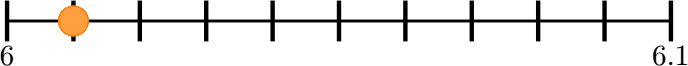
\includegraphics[width=180px]{../images/recta_num_6.01.png}  \hfill \fillin[\fbox{6.01}][0in] \\
				\part 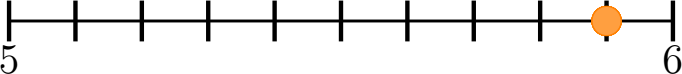
\includegraphics[width=180px]{../images/recta_num_5.9.png}   \hfill \fillin[\fbox{5.9 }][0in] \\
				\part 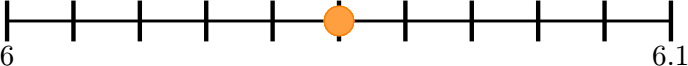
\includegraphics[width=180px]{../images/recta_num_6.05.png}  \hfill \fillin[\fbox{6.05}][0in] \\
				\part 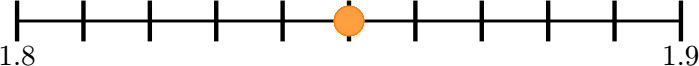
\includegraphics[width=180px]{../images/recta_num_1.85.png}  \hfill \fillin[\fbox{1.85}][0in] \\
				\part 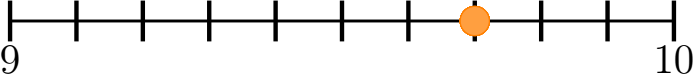
\includegraphics[width=180px]{../images/recta_num_9.7.png}   \hfill \fillin[\fbox{9.7 }][0in] \\
				\part 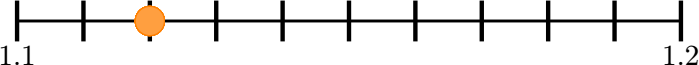
\includegraphics[width=180px]{../images/recta_num_1.12.png}  \hfill \fillin[\fbox{1.12}][0in] \\
				\part 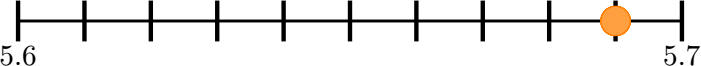
\includegraphics[width=180px]{../images/recta_num_5.69.png}  \hfill \fillin[\fbox{5.69}][0in] \\
				\part 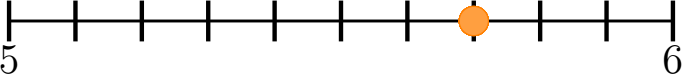
\includegraphics[width=180px]{../images/recta_num_5.7.png}   \hfill \fillin[\fbox{5.7 }][0in] \\
				\part 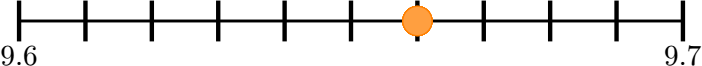
\includegraphics[width=180px]{../images/recta_num_9.66.png}  \hfill \fillin[\fbox{9.66}][0in] \\
				\part 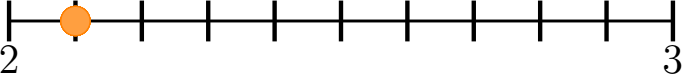
\includegraphics[width=180px]{../images/recta_num_2.1.png}   \hfill \fillin[\fbox{2.1 }][0in] \\
			\end{parts}
		\end{multicols}
	}

	% \subsection*{\ifprintanswers{Porcentaje como decimales             }

	\questionboxed[2]{Escribe los siguientes porcentajes como números decimales:

		\begin{multicols}{4}
			\begin{parts}
				\part $14\%=$ \fillin[\fbox{0.14}][0cm] \\
				\part $73\%=$ \fillin[\fbox{0.73}][0cm] \\
				\part $15\%=$ \fillin[\fbox{0.15}][0cm] \\
				\part $85\%=$ \fillin[\fbox{0.85}][0cm] \\
				\part $91\%=$ \fillin[\fbox{0.91}][0cm] \\
				\part $19\%=$ \fillin[\fbox{0.19}][0cm] \\
				\part $ 9\%=$ \fillin[\fbox{0.09}][0cm] \\
				\part $42\%=$ \fillin[\fbox{0.42}][0cm] \\
				\part $25\%=$ \fillin[\fbox{0.25}][0cm] \\
				\part $ 3\%=$ \fillin[\fbox{0.03}][0cm] \\
				\part $ 8\%=$ \fillin[\fbox{0.08}][0cm] \\
				\part $ 2\%=$ \fillin[\fbox{0.02}][0cm] \\
			\end{parts}
		\end{multicols}
	}

	% \subsection*{\ifprintanswers{Porcentaje de números                 }

	\questionboxed[2]{Calcula los porentajes de los siguientes números:

		\begin{multicols}{2}
			\begin{parts}
				\part ¿Cuál es el 80\% de 660?   \hfill \fillin[\fbox{528}][0cm]
				\part ¿Cuál es el 20\% de 50?    \hfill \fillin[\fbox{10}][0cm]
				\part ¿Cuál es el 50\% de 862?   \hfill \fillin[\fbox{431}][0cm]
				\part ¿Cuál es el 30\% de 300?   \hfill \fillin[\fbox{90}][0cm]
				\part ¿Cuál es el 20\% de 415?   \hfill \fillin[\fbox{83}][0cm]
				\part ¿Cuál es el 12\% de 338?   \hfill \fillin[\fbox{40.56}][0cm]
				\part ¿Cuál es el 15\% de 711?   \hfill \fillin[\fbox{106.65}][0cm]
				\part ¿Cuál es el 80\% de 1260?  \hfill \fillin[\fbox{1008}][0cm]
			\end{parts}
		\end{multicols}
	}

	% \subsection*{\ifprintanswers{Conversión de decimales a fracciones  }

	\questionboxed[2]{Convierte los siguientes números decimales a una fracción simplificada a su mínima expresión:

		\begin{multicols}{4}
			\begin{parts}
				\part $0.248=$ \fillin[\fbox{$\dfrac{31}{125}$}][0cm]
				\part $0.46=$  \fillin[\fbox{$\dfrac{23}{50}$}][0cm]
				\part $0.24=$  \fillin[\fbox{$\dfrac{6}{25}$}][0cm]
				\part $0.9=$   \fillin[\fbox{$\dfrac{9}{10}$}][0cm]
				\part $0.115=$ \fillin[\fbox{$\dfrac{23}{200}$}][0cm]
				\part $0.66=$  \fillin[\fbox{$\dfrac{33}{50}$}][0cm]
				\part $0.56=$  \fillin[\fbox{$\dfrac{14}{25}$}][0cm]
				\part $0.58=$  \fillin[\fbox{$\dfrac{29}{50}$}][0cm]
			\end{parts}
		\end{multicols}
	}

	% \subsection*{\ifprintanswers{Conversión de fracciones a decimales  }  

	\questionboxed[2]{Convierte las siguientes fracciones a decimal:

		\begin{multicols}{5}
			\begin{parts}
				\part $\dfrac{2}{9} =$   \fillin[\fbox{$0.\overline{2}$}][0cm]\\
				\part $\dfrac{1}{4} =$   \fillin[\fbox{$0.25$}][0cm]\\
				\part $\dfrac{2}{3} =$   \fillin[\fbox{$0.\overline{6}$}][0cm]\\
				\part $\dfrac{7}{8} =$   \fillin[\fbox{$0.875$}][0cm]\\
				\part $\dfrac{1}{9} =$   \fillin[\fbox{$0.\overline{1}$}][0cm]\\
				\part $\dfrac{6}{8} =$   \fillin[\fbox{$0.75$}][0cm]\\
				\part $\dfrac{7}{20}=$   \fillin[\fbox{$0.35$}][0cm]\\
				\part $\dfrac{5}{8} =$   \fillin[\fbox{$0.625$}][0cm]\\
				\part $\dfrac{2}{10}=$   \fillin[\fbox{$0.2$}][0cm]\\
				\part $\dfrac{5}{6} =$   \fillin[\fbox{$0.8\overline{3}$}][0cm]\\
			\end{parts}
		\end{multicols}
	}


	\addcontentsline{toc}{subsection}{Introducción a las fracciones}
	\subsection*{Introducción a las fracciones}

	% \subsection*{\ifprintanswers{Clasificación de fracciones           }
	\questionboxed[2]{Clasifica las siguientes fracciones en propias, impropias o mixtas:

		\begin{multicols}{4}
			\begin{parts}
				\part $\dfrac{5}{6}$   \fillin[Propia][1in]     \\[0.5em]
				\part $5\dfrac{5}{11}$ \fillin[Mixta][1in]      \\[0.5em]
				\part $\dfrac{13}{12}$   \fillin[Impropia][1in] \\[0.5em]
				\part $1\dfrac{2}{15}$  \fillin[Mixta][1in]     \\[0.5em]
				\part $\dfrac{42}{43}$   \fillin[Propia][1in]   \\[0.5em]
				\part $\dfrac{16}{9}$   \fillin[Impropia][1in]  \\[0.5em]
				\part $\dfrac{7}{3}$   \fillin[Impropia][1in]   \\[0.5em]
				\part $3\dfrac{2}{9}$  \fillin[Mixta][1in]      \\[0.5em]
				\part $\dfrac{3}{2}$   \fillin[Impropia][1in]   \\[0.5em]
				\part $1\dfrac{2}{3}$  \fillin[Mixta][1in]      \\[0.5em]
				\part $\dfrac{7}{8}$   \fillin[Propia][1in]     \\[0.5em]
				\part $\dfrac{6}{5}$   \fillin[Impropia][1in]   \\[0.5em]
			\end{parts}
		\end{multicols}
	}

	% \subsection*{\ifprintanswers{Nombre de fracciones                       }\else{}\fi}

	\questionboxed[2]{Escribe la fracción que corresponda en cada inciso:

		\begin{parts}
			\part ¿Cómo se escribe numéricamente la fracción \textbf{siete catorceavos}?    \fillin[$\dfrac{7}{14}$][0in]
			\part ¿Cómo se escribe numéricamente la fracción \textbf{ocho onceavos}?   \fillin[$\dfrac{8}{11}$][0in]
			\part ¿Cómo se escribe numéricamente la fracción \textbf{doce séptimos}?    \fillin[$\dfrac{12}{7}$][0in]
			\part ¿Cómo se escribe numéricamente la fracción \textbf{nueve treceavos}?     \fillin[$\dfrac{9}{13}$][0in]
		\end{parts}
	}

	% \subsection*{\ifprintanswers{Representación de fracciones}\else{}\fi}
	\questionboxed[2]{Escribe sobre la línea la fracción que representa cada imagen:

		\begin{multicols}{4}
			\begin{parts}
				\part 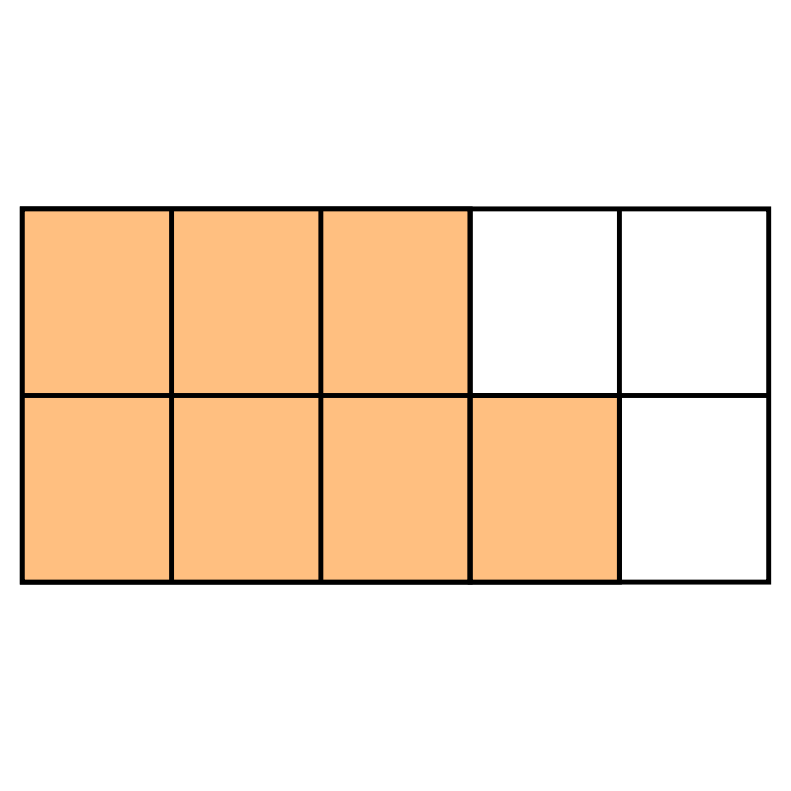
\includegraphics[width=50px]{../images/imagen_frac_5prim_7|10.png} \fillin[\fbox{$\dfrac{7}{10}$}][0in] \\[-0.5em]
				\part 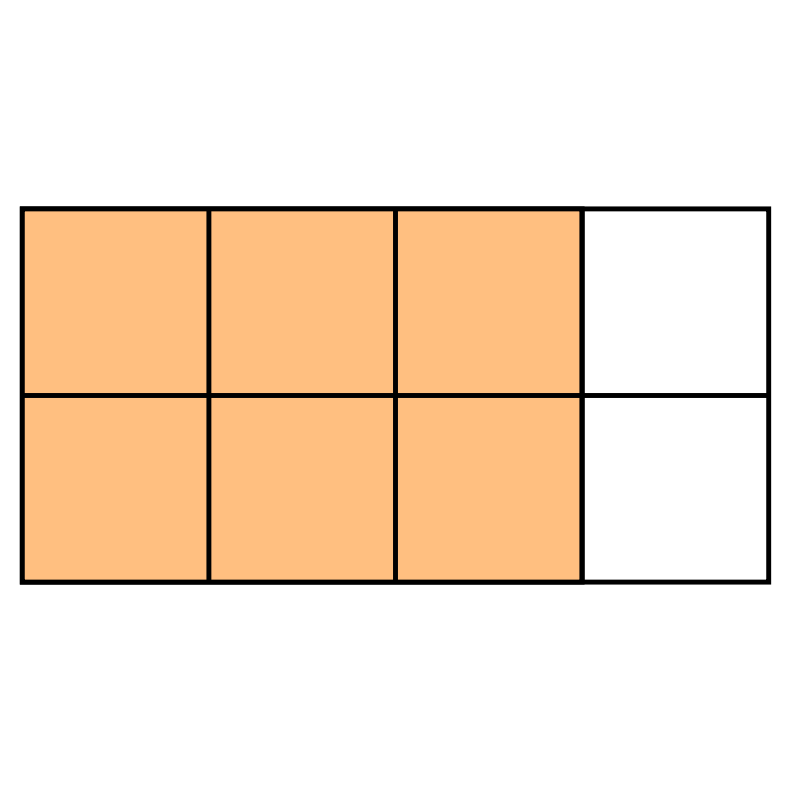
\includegraphics[width=50px]{../images/imagen_frac_5prim_6|8.png} \fillin[\fbox{$\dfrac{6}{8}$}][0in] \\[-0.5em]
				\part 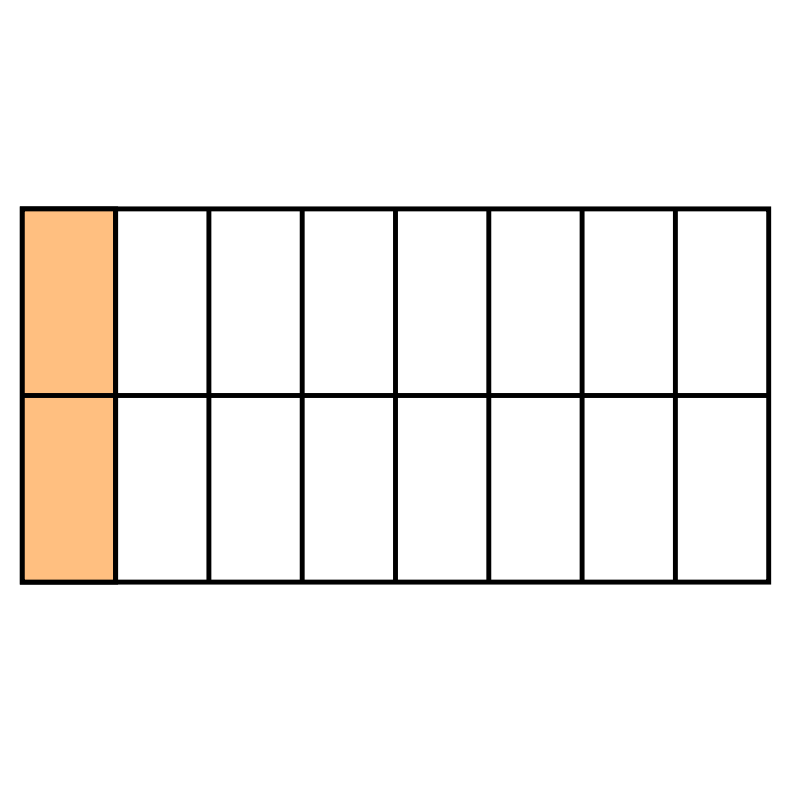
\includegraphics[width=50px]{../images/imagen_frac_5prim_2|16.png} \fillin[\fbox{$\dfrac{2}{16}$}][0in] \\[-0.5em]
				\part 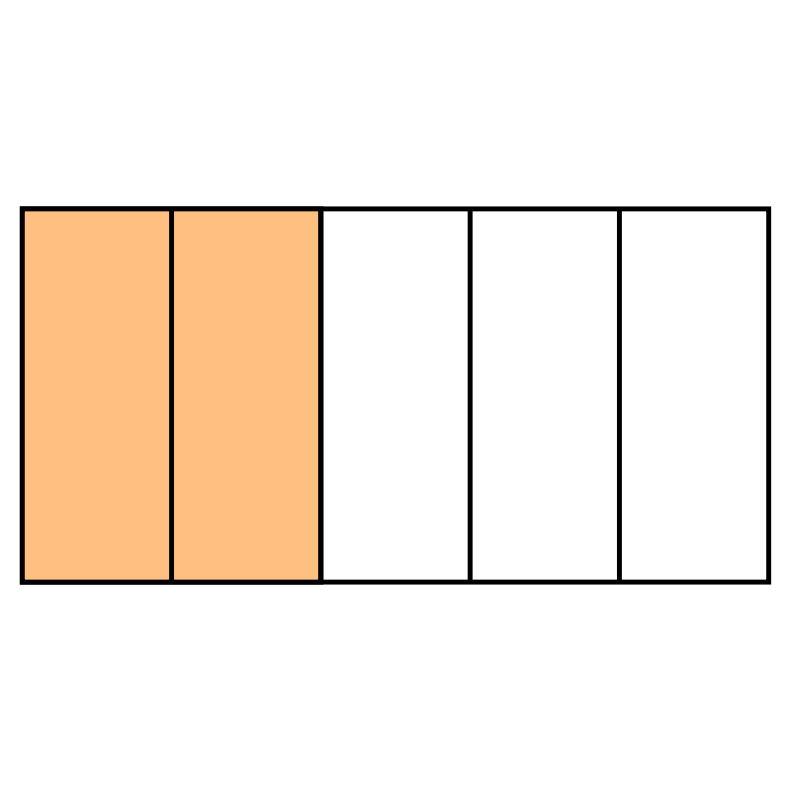
\includegraphics[width=50px]{../images/imagen_frac_5prim_2|5.png} \fillin[\fbox{$\dfrac{2}{5}$}][0in] \\[-0.5em]
				\part 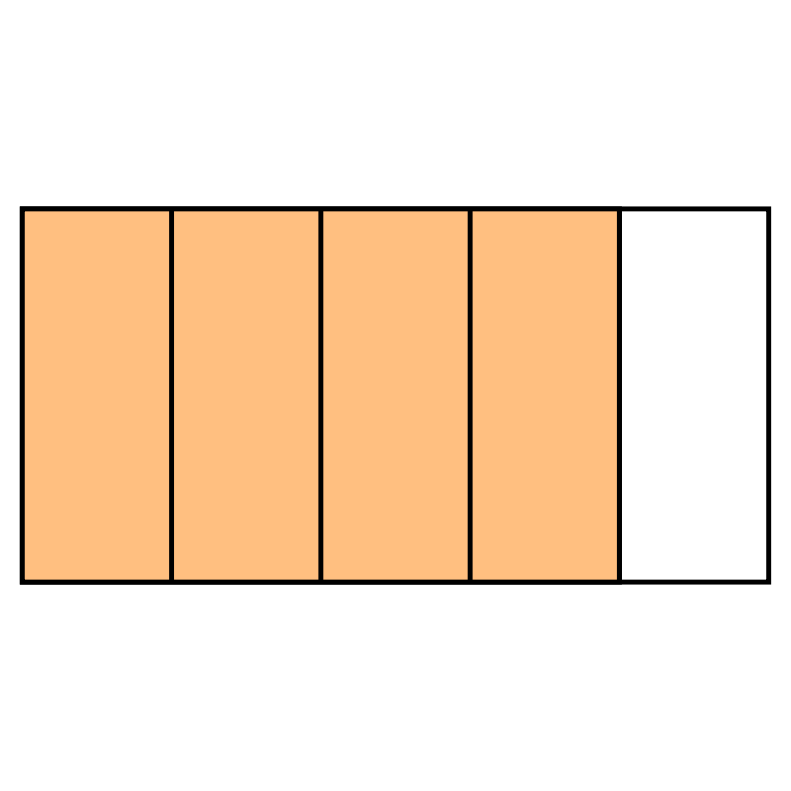
\includegraphics[width=50px]{../images/imagen_frac_5prim_4|5.png} \fillin[\fbox{$\dfrac{4}{5}$}][0in] \\[-0.5em]
				\part 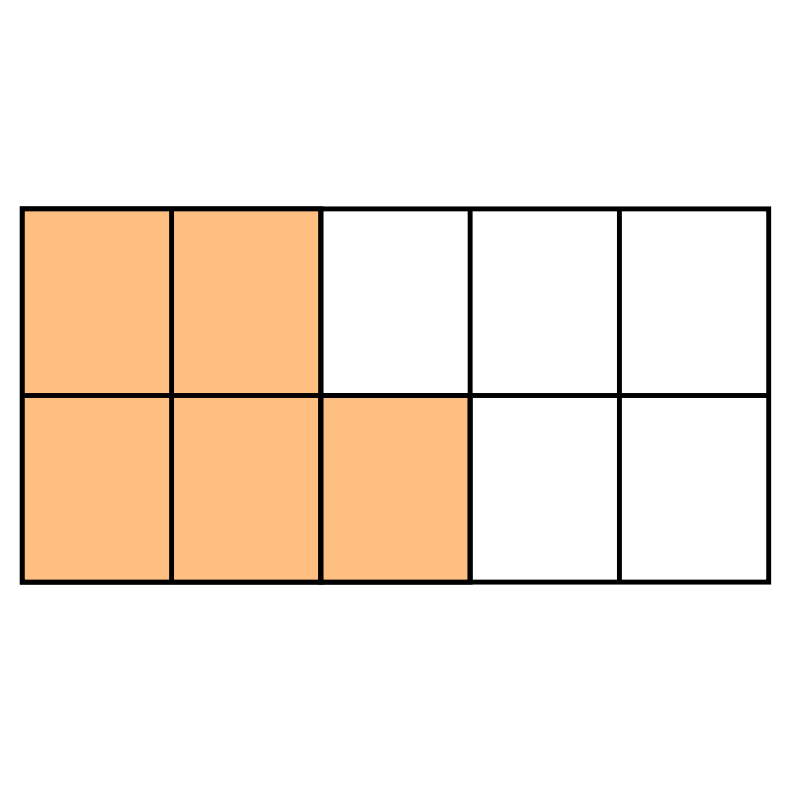
\includegraphics[width=50px]{../images/imagen_frac_5prim_5|10.png} \fillin[\fbox{$\dfrac{5}{10}$}][0in] \\[-0.5em]
				\part 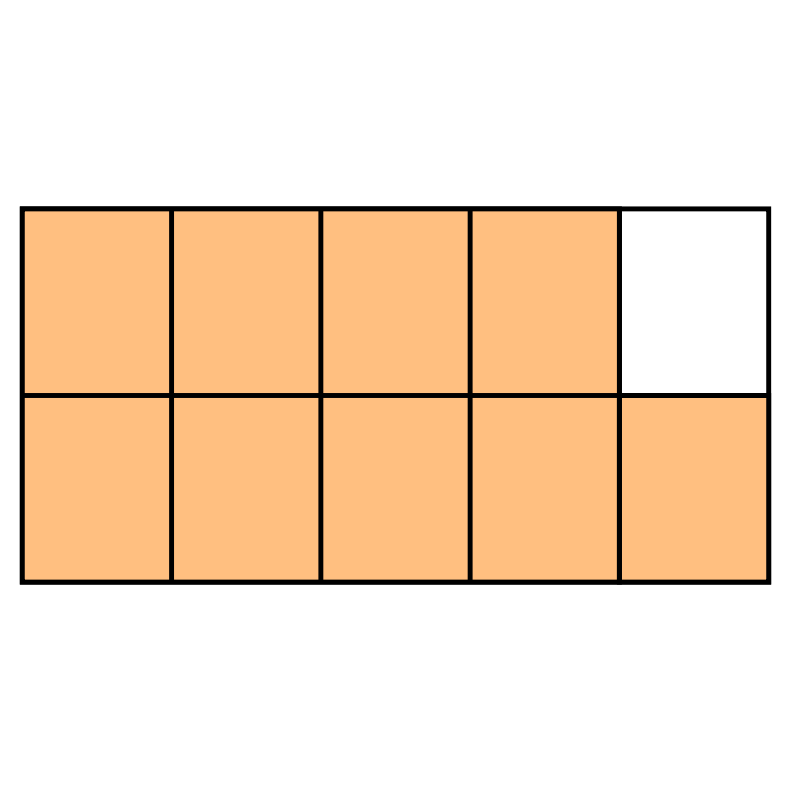
\includegraphics[width=50px]{../images/imagen_frac_5prim_9|10.png} \fillin[\fbox{$\dfrac{9}{10}$}][0in] \\[-0.5em]
				\part 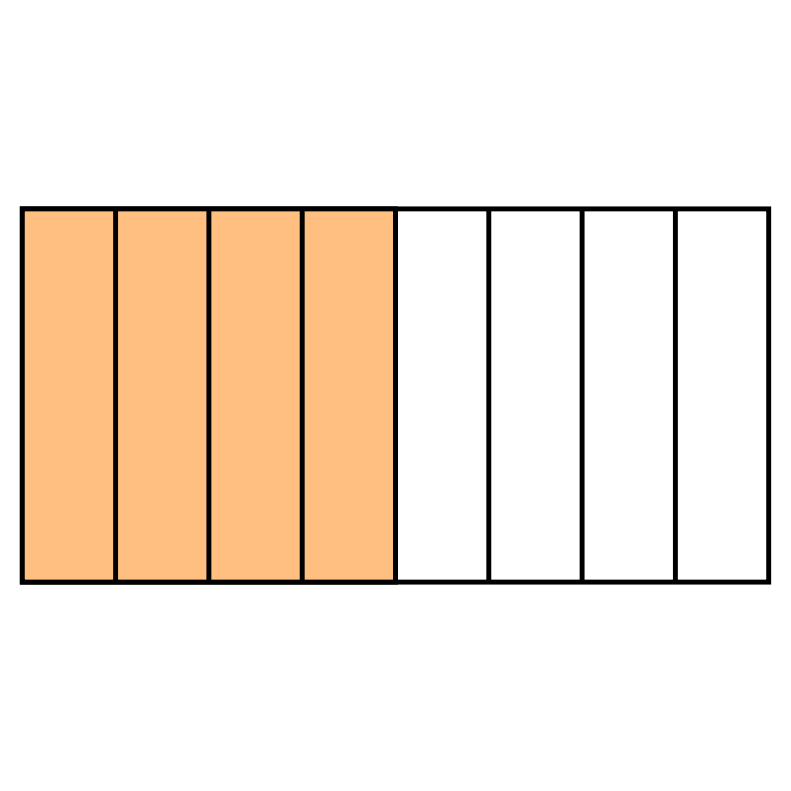
\includegraphics[width=50px]{../images/imagen_frac_5prim_4|8.png} \fillin[\fbox{$\dfrac{4}{8}$}][0in] \\[-0.5em]
				\part 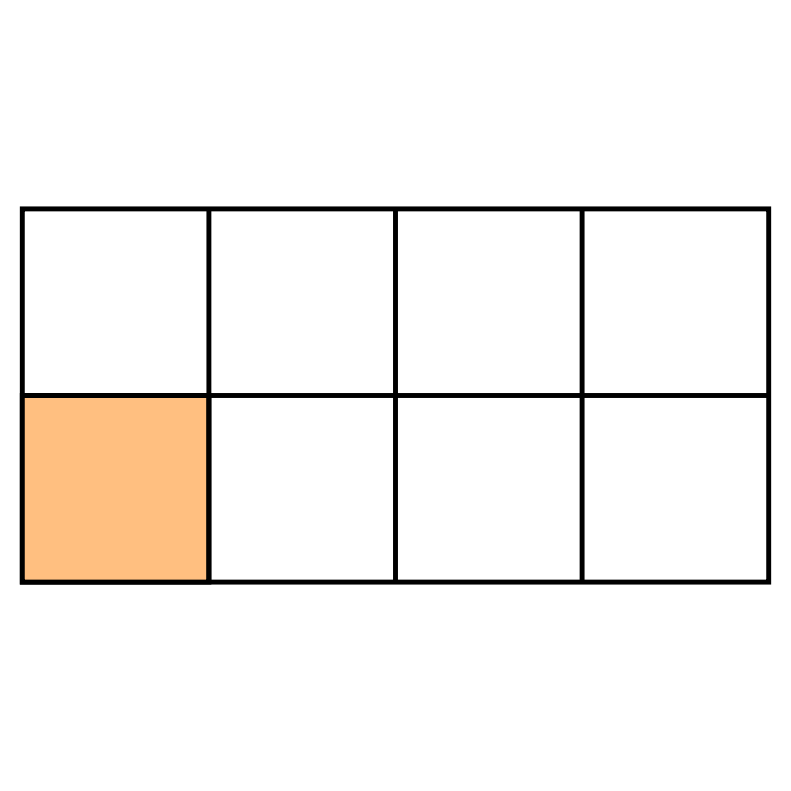
\includegraphics[width=50px]{../images/imagen_frac_5prim_1|8.png} \fillin[\fbox{$\dfrac{1}{8}$}][0in] \\[-0.5em]
				\part 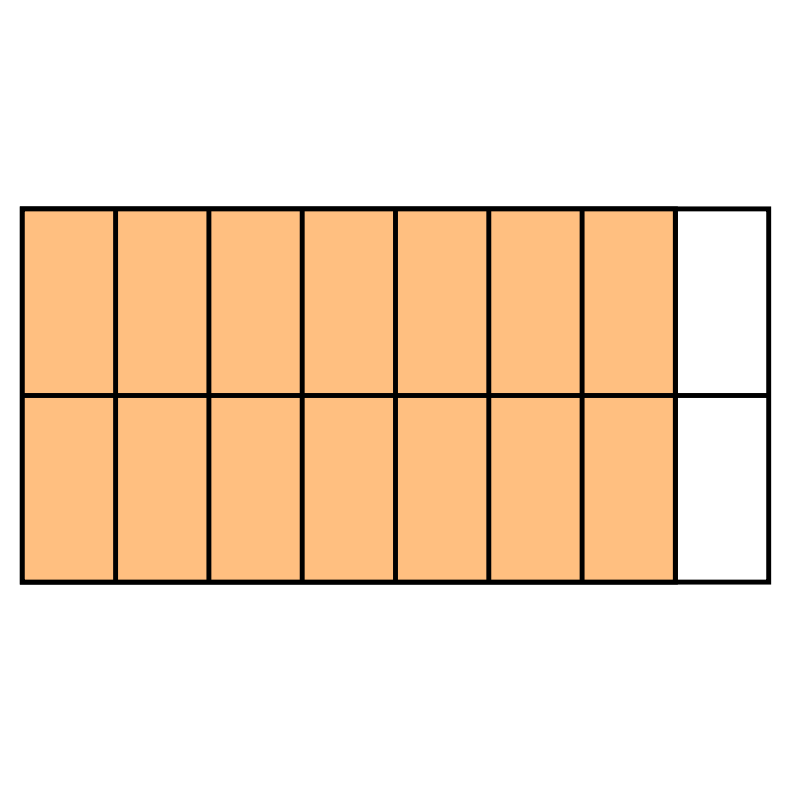
\includegraphics[width=50px]{../images/imagen_frac_5prim_14|16.png} \fillin[\fbox{$\dfrac{14}{16}$}][0in] \\[-0.5em]
				\part 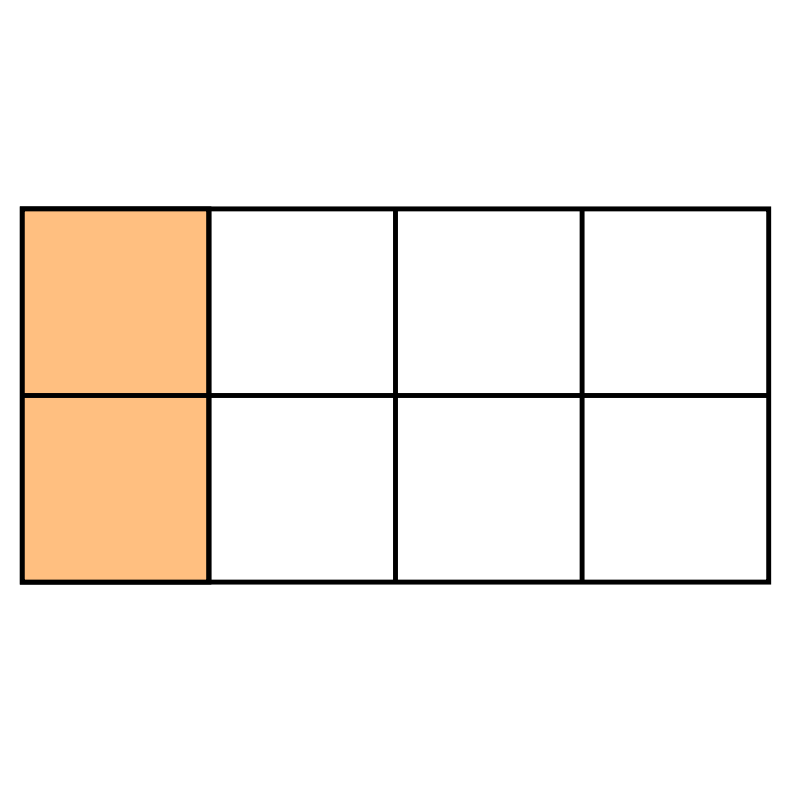
\includegraphics[width=50px]{../images/imagen_frac_5prim_2|8.png} \fillin[\fbox{$\dfrac{2}{8}$}][0in] \\[-0.5em]
				\part 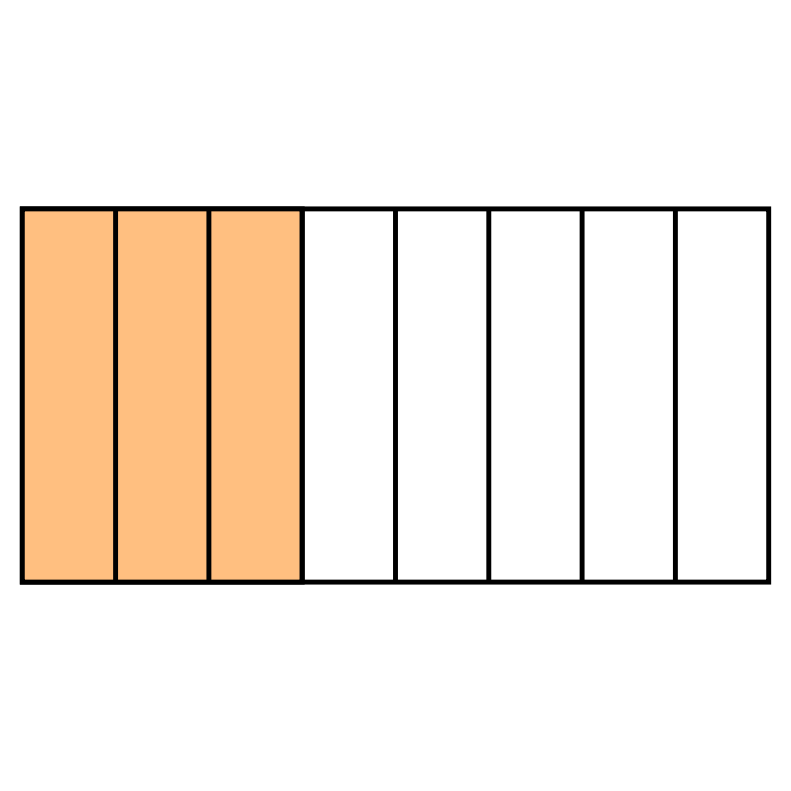
\includegraphics[width=50px]{../images/imagen_frac_5prim_3|8.png} \fillin[\fbox{$\dfrac{3}{8}$}][0in] \\[-0.5em]
				\part 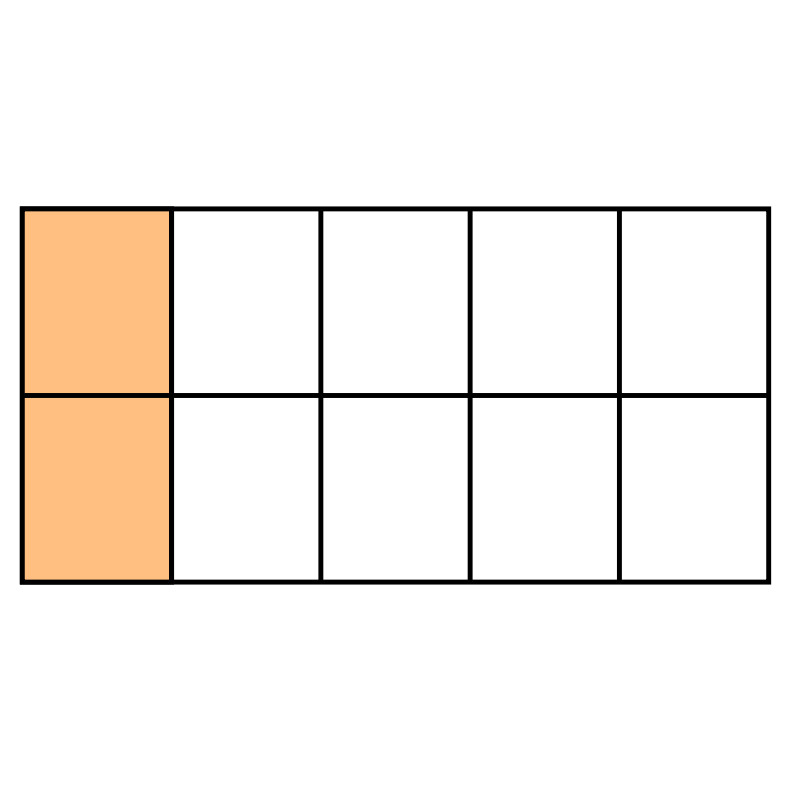
\includegraphics[width=50px]{../images/imagen_frac_5prim_2|10.png} \fillin[\fbox{$\dfrac{2}{10}$}][0in] \\[-0.5em]
				\part 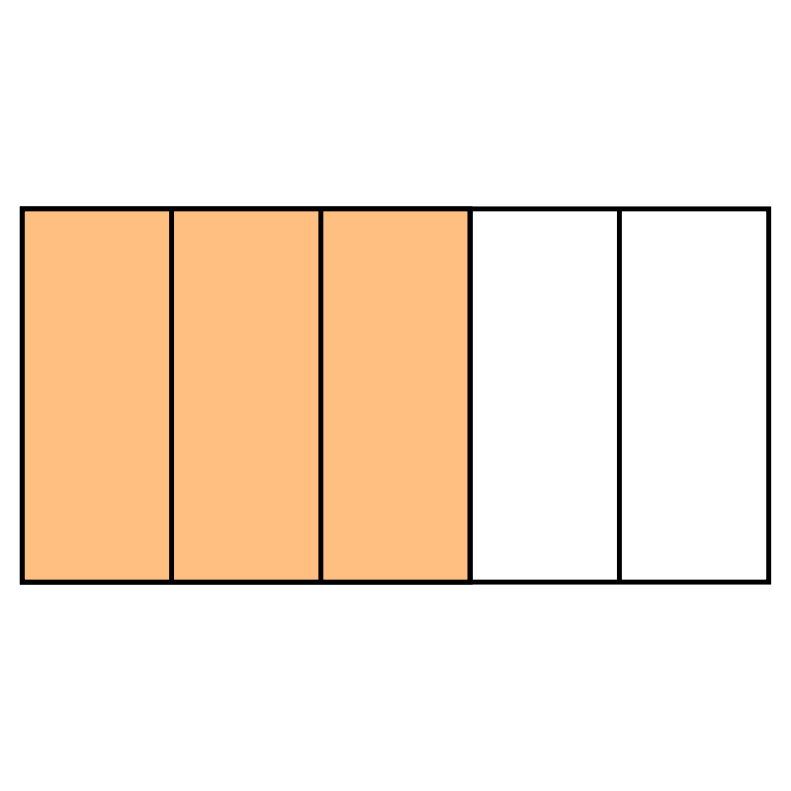
\includegraphics[width=50px]{../images/imagen_frac_5prim_3|5.png} \fillin[\fbox{$\dfrac{3}{5}$}][0in] \\[-0.5em]
				\part 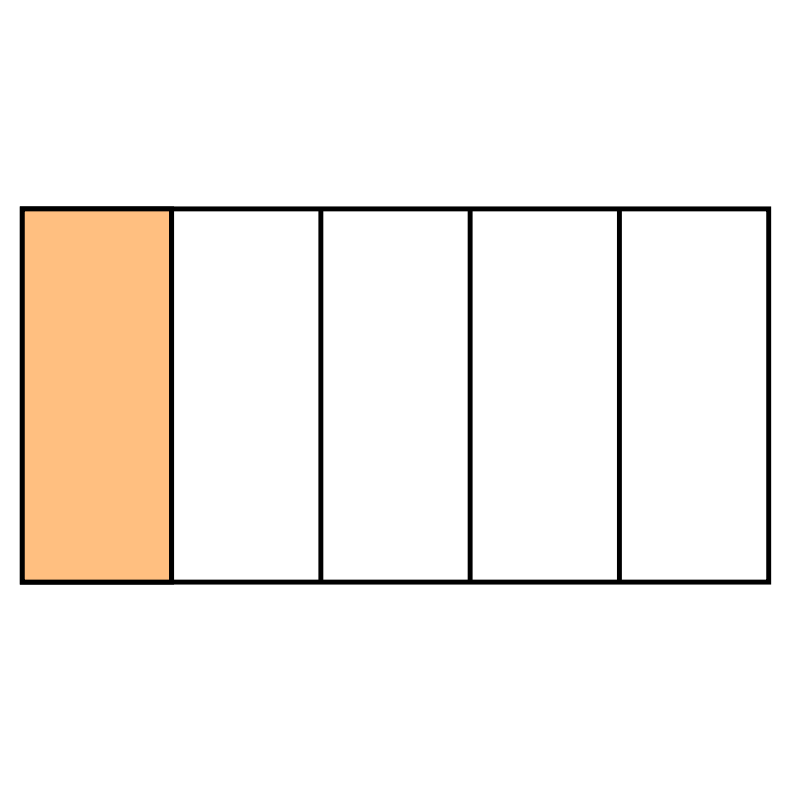
\includegraphics[width=50px]{../images/imagen_frac_5prim_1|5.png} \fillin[\fbox{$\dfrac{1}{5}$}][0in] \\[-0.5em]
				\part 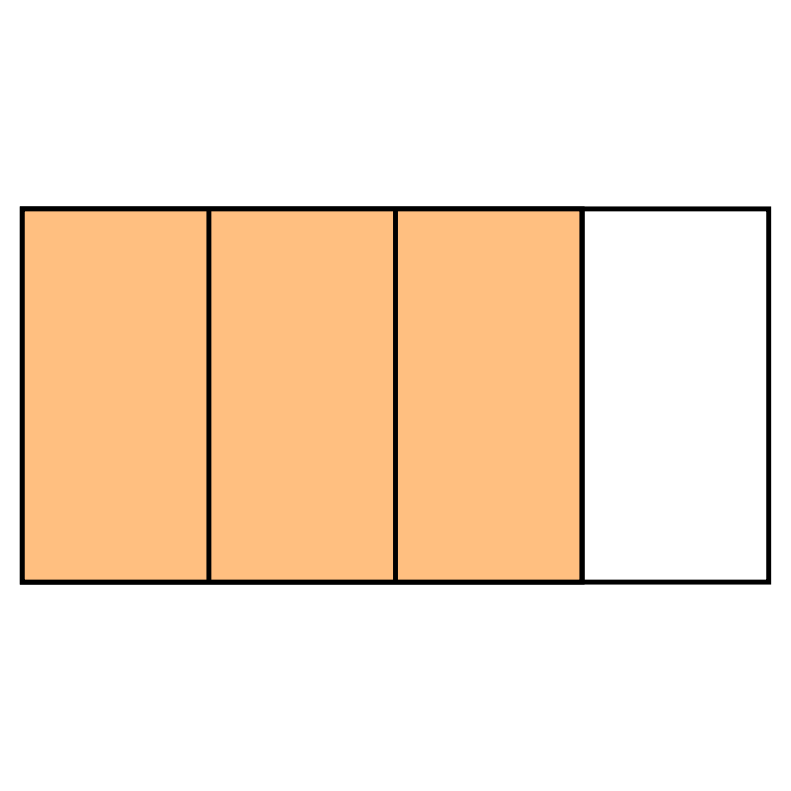
\includegraphics[width=50px]{../images/imagen_frac_5prim_3|4.png} \fillin[\fbox{$\dfrac{3}{4}$}][0in] \\[-0.5em]


			\end{parts}
		\end{multicols}
	}


	% \subsection*{\ifprintanswers{Fracciones en la recta numérica}
	% \subsection*{\ifprintanswers{Decimales en la recta númerica        }
	\questionboxed[2]{Escribe la fracción que representa el punto en la recta numérica de cada imagen:

		\begin{multicols}{2}
			\begin{parts}
				\part 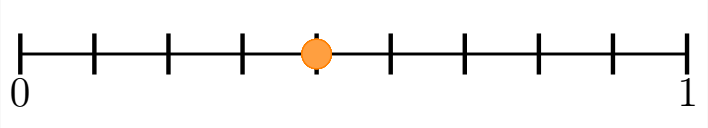
\includegraphics[width=180px]{../images/recta_num_frac4|9.png}   \hfill \fillin[\fbox{$\dfrac{ 4}{9 }$}][0in] \\
				\part 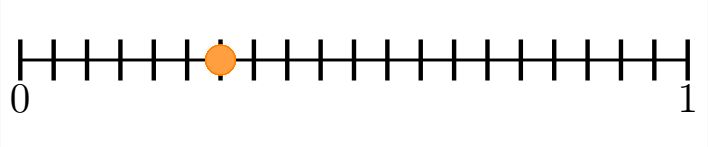
\includegraphics[width=180px]{../images/recta_num_frac6|20.png}  \hfill \fillin[\fbox{$\dfrac{ 6}{20}$}][0in] \\
				\part 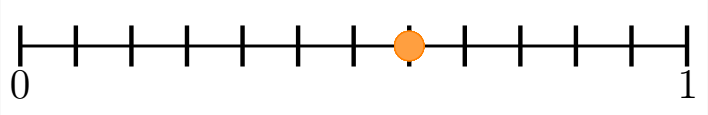
\includegraphics[width=180px]{../images/recta_num_frac7|12.png}  \hfill \fillin[\fbox{$\dfrac{ 7}{12}$}][0in] \\
				\part 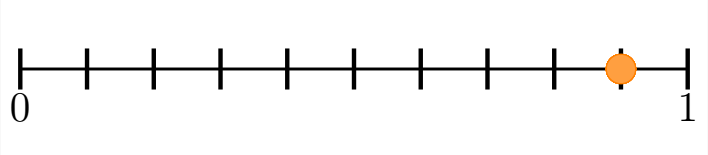
\includegraphics[width=180px]{../images/recta_num_frac9|10.png}  \hfill \fillin[\fbox{$\dfrac{ 9}{10}$}][0in] \\
				\part 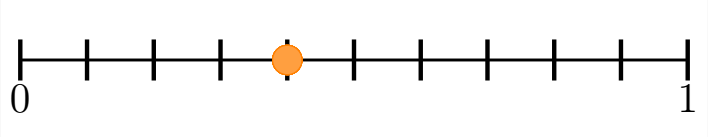
\includegraphics[width=180px]{../images/recta_num_frac4|10.png}  \hfill \fillin[\fbox{$\dfrac{ 4}{10}$}][0in] \\
				\part 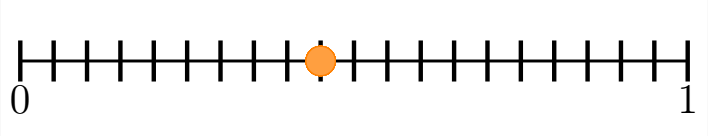
\includegraphics[width=180px]{../images/recta_num_frac9|20.png}  \hfill \fillin[\fbox{$\dfrac{ 9}{20}$}][0in] \\
				\part 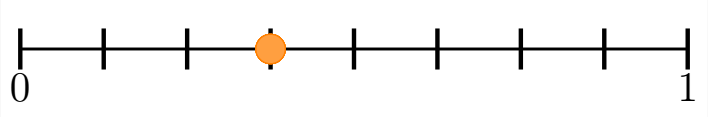
\includegraphics[width=180px]{../images/recta_num_frac3|8.png}   \hfill \fillin[\fbox{$\dfrac{ 3}{8 }$}][0in] \\
				\part 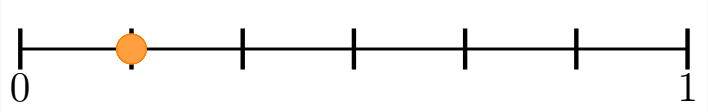
\includegraphics[width=180px]{../images/recta_num_frac1|6.png}   \hfill \fillin[\fbox{$\dfrac{ 1}{6 }$}][0in] \\
				\part 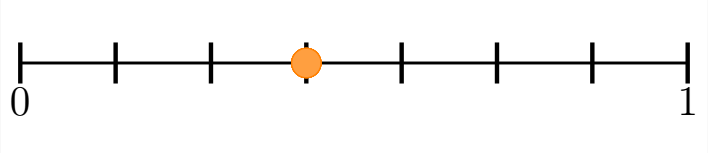
\includegraphics[width=180px]{../images/recta_num_frac3|7.png}   \hfill \fillin[\fbox{$\dfrac{ 3}{7 }$}][0in] \\
				\part 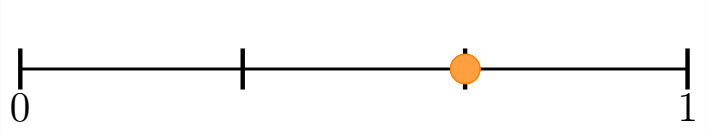
\includegraphics[width=180px]{../images/recta_num_frac2|3.png}   \hfill \fillin[\fbox{$\dfrac{ 2}{3 }$}][0in] \\
			\end{parts}
		\end{multicols}
	}



	% \subsection*{\ifprintanswers{Conversión de fracciones}
	\questionboxed[2]{Convierte la siguientes fracciones mixtas a impropias y viseversa:

		\begin{multicols}{3}
			\begin{parts}
				\part $4\dfrac{2}{3}= $  \fillin[$\dfrac{14}{3}$][0in]\\[0.5em]
				\part $\dfrac{13}{3}= $  \fillin[$4\dfrac{1}{3}$][0in]\\[0.5em]
				\part $2\dfrac{3}{10}= $ \fillin[$\dfrac{23}{10}$][0in]\\[0.5em]
				\part $\dfrac{43}{10}= $ \fillin[$4\dfrac{3}{10}$][0in]\\[0.5em]
				\part $5\dfrac{1}{5}= $  \fillin[$\dfrac{26}{5}$][0in]\\[0.5em]
				\part $\dfrac{51}{5}= $  \fillin[$10\dfrac{1}{5}$][0in]\\[0.5em]
			\end{parts}
		\end{multicols}
	}



	\addcontentsline{toc}{subsection}{Suma y resta de fracciones}
	\subsection*{Suma y resta de fracciones}
	% \subsection*{\ifprintanswers{Simplificación de fracciones          }
	\questionboxed[2]{Simplifica a su mínima expresión las siguientes fracciones usando el máximo común divisor:

		\begin{multicols}{5}
			\begin{parts}
				\part $\dfrac{12}{48}= $  \fillin[$\dfrac{1}{4}$][0in]\\[0.5em]
				\part $\dfrac{6}{24}= $  \fillin[$\dfrac{1}{4}$][0in]\\[0.5em]
				\part $\dfrac{16}{36}= $  \fillin[$\dfrac{4}{9}$][0in]\\[0.5em]
				\part $\dfrac{4}{40}= $  \fillin[$\dfrac{1}{10}$][0in]\\[0.5em]
				\part $\dfrac{4}{20}= $  \fillin[$\dfrac{1}{5}$][0in]\\[0.5em]
				\part $\dfrac{2}{30}= $  \fillin[$\dfrac{1}{15}$][0in]\\[0.5em]
				\part $\dfrac{6}{36}= $  \fillin[$\dfrac{1}{6}$][0in]\\[0.5em]
				\part $\dfrac{5}{25}= $  \fillin[$\dfrac{1}{5}$][0in]\\[0.5em]
				\part $\dfrac{6}{30}= $  \fillin[$\dfrac{1}{5}$][0in]\\[0.5em]
				\part $\dfrac{2}{12}= $  \fillin[$\dfrac{1}{6}$][0in]\\[0.5em]
				\part $\dfrac{4}{16}= $  \fillin[$\dfrac{1}{4}$][0in]\\[0.5em]
				\part $\dfrac{15}{20}= $  \fillin[$\dfrac{3}{4}$][0in]\\[0.5em]
				\part $\dfrac{5}{50}= $  \fillin[$\dfrac{1}{10}$][0in]\\[0.5em]
				\part $\dfrac{6}{10}= $  \fillin[$\dfrac{3}{5}$][0in]\\[0.5em]
				\part $\dfrac{3}{18}= $  \fillin[$\dfrac{1}{6}$][0in]\\[0.5em]
			\end{parts}
		\end{multicols}
	}


	% \subsection*{\ifprintanswers{Suma y resta con denominadores iguales}
	% \subsection*{\ifprintanswers{Suma con denominadores diferentes     }
	% \subsection*{\ifprintanswers{Resta con denominadores diferentes    }
	% \subsection*{\ifprintanswers{Sumas y restas con fracciones mixtas  }

	\questionboxed[4]{Realiza las siguientes operaciones de suma y resta de fracciones:

		\begin{multicols}{3}
			\begin{parts}
				\part $\dfrac{3}{5}+\dfrac{4}{5}=$ \fillin[$\dfrac{7}{5} = 1\dfrac{2}{5}$][0in] \\[1em]
				\part $\dfrac{3}{10}+\dfrac{4}{5}=$ \fillin[$\dfrac{11}{10} = 1\dfrac{1}{10}$][0in] \\[1em]
				\part $\dfrac{9}{10}+\dfrac{2}{3}=$ \fillin[$1\dfrac{17}{30}$][0in] \\[1em]
				\part $\dfrac{13}{6}-\dfrac{5}{6}=$ \fillin[$\dfrac{8}{6}=\dfrac{4}{3}$][0in] \\[1em]
				\part $1\dfrac{1}{2}+1\dfrac{2}{3}=$ \fillin[$3\dfrac{1}{6}$][0in] \\[1em]
				\part $\dfrac{3}{4}-\dfrac{2}{5}=$ \fillin[$\dfrac{7}{20}$][0in] \\[1em]
				\part $\dfrac{5}{6}+\dfrac{1}{12}=$ \fillin[$\dfrac{11}{12}$][0in] \\[1em]
				\part $\dfrac{12}{7}-\dfrac{5}{7}=$ \fillin[$\dfrac{7}{7}=1$][0in] \\[1em]
				\part $\dfrac{2}{3}-\dfrac{2}{5}=$ \fillin[$\dfrac{4}{15}$][0in] \\[1em]
				\part $2\dfrac{1}{2}-1\dfrac{1}{3}=$ \fillin[$1\dfrac{1}{6}$][0in] \\[1em]
				\part $\dfrac{1}{3}-\dfrac{1}{4}=$ \fillin[$\dfrac{1}{12}$][0in] \\[1em]
				\part $1\dfrac{1}{8}+1\dfrac{7}{8}=$ \fillin[$2\dfrac{8}{8} = 3$][0in] \\[1em]
				\part $\dfrac{3}{8}+\dfrac{7}{10}=$ \fillin[$\dfrac{43}{40} = 1\dfrac{3}{40}$][0in] \\[1em]
				\part $\dfrac{3}{4}-\dfrac{1}{8}=$ \fillin[$\dfrac{5}{8}$][0in] \\[1em]
				\part $3\dfrac{3}{4}-2\dfrac{2}{3}=$ \fillin[$1\dfrac{1}{12}$][0in] \\[1em]
			\end{parts}
		\end{multicols}
	}


	\addcontentsline{toc}{subsection}{Multiplicación y división de fracciones}
	\subsection*{Multiplicación y división de fracciones}
	% \subsection*{\ifprintanswers{Multiplicación de fracciones          }
	% \subsection*{\ifprintanswers{División de fracciones                }
	% \subsection*{\ifprintanswers{Multiplicación y división con enteros }
	% \subsection*{\ifprintanswers{Multiplicación con fracciones mixtas  }
	% \subsection*{\ifprintanswers{División con fracciones mixtas        }

	\questionboxed[5]{Realiza las siguientes operaciones de multiplicación y división de fracciones (Expresa tu resultadocomo una \textbf{fracción simplificada}):

		\begin{multicols}{4}
			\begin{parts}
				\part $\dfrac{7}{9}\times\dfrac{12}{17}=$ \fillin[$\dfrac{28}{51}$][0in]   \\[1em]
				\part $\dfrac{2}{7}\divisionsymbol\dfrac{2}{5}=$ \fillin[$\dfrac{5}{7}$][0in]   \\[1em]
				\part $3\times\dfrac{5}{4}=$ \fillin[$\dfrac{15}{4}$][0in]   \\[1em]
				\part $1\dfrac{1}{4}\times 4\dfrac{5}{8}=$ \fillin[$\dfrac{185}{32}$][0in]   \\[1em]
				\part $\dfrac{5}{6}\times\dfrac{4}{5}=$ \fillin[$\dfrac{2}{3}$][0in]   \\[1em]
				\part $\dfrac{4}{7}\divisionsymbol\dfrac{5}{6}=$ \fillin[$\dfrac{24}{35}$][0in]   \\[1em]
				\part $\dfrac{7}{6}\times 6=$ \fillin[$\dfrac{21}{2}$][0in]   \\[1em]
				\part $3\dfrac{1}{3}\times 2\dfrac{2}{5}=$ \fillin[$8$][0in]   \\[1em]
				\part $\dfrac{3}{7}\times\dfrac{5}{6}=$ \fillin[$\dfrac{5}{14}$][0in]   \\[1em]
				\part $\dfrac{7}{8}\divisionsymbol\dfrac{5}{4}=$ \fillin[$\dfrac{7}{10}$][0in]   \\[1em]
				\part $\dfrac{2}{5}\divisionsymbol 5=$ \fillin[$\dfrac{2}{25}$][0in]   \\[1em]
				\part $6\dfrac{1}{2}\divisionsymbol 1\dfrac{5}{7}=$ \fillin[$\dfrac{91}{24}$][0in]   \\[1em]
				\part $\dfrac{5}{8}\times\dfrac{4}{5}=$ \fillin[$\dfrac{1}{2}$][0in]   \\[1em]
				\part $\dfrac{6}{7}\divisionsymbol\dfrac{1}{3}=$ \fillin[$\dfrac{18}{7}$][0in]   \\[1em]
				\part $4\divisionsymbol\dfrac{3}{5}=$ \fillin[$\dfrac{20}{3}$][0in]   \\[1em]
				\part $2\dfrac{2}{3}\divisionsymbol 1\dfrac{3}{4}=$ \fillin[$\dfrac{32}{21}$][0in]   \\[1em]
			\end{parts}
		\end{multicols}
	}


	\addcontentsline{toc}{subsection}{MCD y MCM}
	\subsection*{MCD y MCM}


	% \subsection*{\ifprintanswers{Fracciones equivalentes               }

	\questionboxed[2]{Indica si las siguientes fracciones son equivalentes o no:

		\begin{multicols}{2}
			\begin{parts}

				\part $\dfrac{1}{2}=\dfrac{4}{6}$\qquad
				\begin{oneparcheckboxes}
					\choice Sí
					\CorrectChoice No
				\end{oneparcheckboxes}

				\part $\dfrac{4}{5}=\dfrac{8}{10}$\qquad
				\begin{oneparcheckboxes}
					\CorrectChoice Sí
					\choice No
				\end{oneparcheckboxes}

				\part $\dfrac{1}{8}=\dfrac{4}{16}$\qquad
				\begin{oneparcheckboxes}
					\choice Sí
					\CorrectChoice No
				\end{oneparcheckboxes}

				\part $\dfrac{1}{5}=\dfrac{5}{10}$\qquad
				\begin{oneparcheckboxes}
					\choice Sí
					\CorrectChoice No
				\end{oneparcheckboxes}

				\part $\dfrac{1}{10}=\dfrac{3}{30}$\qquad
				\begin{oneparcheckboxes}
					\CorrectChoice Sí
					\choice No
				\end{oneparcheckboxes}

				\part $\dfrac{1}{4}=\dfrac{2}{4}$\qquad
				\begin{oneparcheckboxes}
					\choice Sí
					\CorrectChoice No
				\end{oneparcheckboxes}

				\part $\dfrac{1}{5}=\dfrac{10}{25}$\qquad
				\begin{oneparcheckboxes}
					\choice Sí
					\CorrectChoice No
				\end{oneparcheckboxes}

				\part $\dfrac{3}{2}=\dfrac{12}{8}$\qquad
				\begin{oneparcheckboxes}
					\CorrectChoice Sí
					\choice No
				\end{oneparcheckboxes}

				\part $\dfrac{3}{6}=\dfrac{1}{3}$\qquad
				\begin{oneparcheckboxes}
					\choice Sí
					\CorrectChoice No
				\end{oneparcheckboxes}

				\part $\dfrac{18}{12}=\dfrac{9}{4}$\qquad
				\begin{oneparcheckboxes}
					\choice Sí
					\CorrectChoice No
				\end{oneparcheckboxes}
			\end{parts}
		\end{multicols}
	}

	% \subsection*{\ifprintanswers{Factores primos                       }

	\questionboxed[2]{Descomponer en factores primos cada uno de los siguientes números:

		\begin{multicols}{3}
			\begin{parts}
				\part $81=$    \fillin[$3 \times 3 \times 3 \times 3$][3.8cm] \\
				\part $34=$    \fillin[$2 \times 17$][3.8cm] \\
				\part $8=$     \fillin[$2 \times 2 \times 2$][3.8cm] \\
				\part $243=$   \fillin[$3 \times 3 \times 3 \times 3 \times 3$][3.8cm] \\
				\part $33=$    \fillin[$3 \times 11$][3.8cm] \\
				\part $150=$   \fillin[$2 \times 3 \times 5 \times 5$][3.8cm] \\
				\part $144=$   \fillin[$2 \times 2 \times 2 \times 2 \times 3 \times 3$][3.8cm] \\
				\part $55=$    \fillin[$5 \times 11$][3.8cm] \\
				\part $125=$   \fillin[$5 \times 5 \times 5$][3.8cm] \\
			\end{parts}
		\end{multicols}
	}

	% \subsection*{\ifprintanswers{Mínimo común múltiplo                 }

	% \subsection*{\ifprintanswers{Máximo común divisor                  }
	\questionboxed[4]{Calcula lo que se te pide en cada inciso:

		% \begin{multicols}{2}
		\begin{parts}
			\part Encuentra el mínimo común múltiplo de 2 y 9.     	\hfill\fillin[El MCM de 2 y 9 es 18.][0in] \\[0.8em]
			\part Encuentra el máximo común divisor de 5 y 15.     	\hfill\fillin[El MCD de 5 y 15 es 5.][0in] \\[0.8em]
			\part Encuentra el máximo común divisor de 33 y 121.   	\hfill\fillin[El MCD de 33 y 121 es 11.][0in] \\[0.8em]
			\part Encuentra el máximo común divisor de 25 y 100.   	\hfill\fillin[El MCD de 25 y 100 es 25.][0in] \\[0.8em]
			\part Encuentra el máximo común divisor de 18 y 36.    	\hfill\fillin[El MCD de 18 y 36 es 18.][0in] \\[0.8em]
			\part Encuentra el mínimo común múltiplo de 4 y 9.     	\hfill\fillin[El MCM de 4 y 9 es 36.][0in] \\[0.8em]
			\part Encuentra el mínimo común múltiplo de 6 y 7.     	\hfill\fillin[El MCM de 6 y 7 es 42.][0in] \\[0.8em]
			\part Encuentra el mínimo común múltiplo de 2, 3 y 4.  	\hfill\fillin[El MCM de 2, 3 y 4 es 12.][0in] \\[0.8em]
			\part Encuentra el máximo común divisor de 2 y 14.     	\hfill\fillin[El MCD de 2 y 14 es 2.][0in] \\[0.8em]
			\part Encuentra el mínimo común múltiplo de 12, 15 y 18.\hfill\fillin[El MCM de 12, 15 y 18 es 180.][0in] \\[0.8em]
		\end{parts}
		% \end{multicols}
	}

	% \subsection*{\ifprintanswers{Simplificación de fracciones          }

	\addcontentsline{toc}{section}{Unidad 3}
	\section*{Unidad 3}
	\addcontentsline{toc}{subsection}{Estadística y gráficas}
	\subsection*{Estadística y gráficas}
	% \subsection*{\ifprintanswers{Mediana    }                                            
	% \subsection*{\ifprintanswers{Moda       }                                            
	% \subsection*{\ifprintanswers{Media      }

	\questionboxed[2]{Determina la mediana y la moda en los siguientes conjuntos de datos:

		\begin{multicols}{2}
			\begin{parts}
				\part 80, 82, 85, 88, 90, 88, 91, 85, 95, 88, 88, 97, 100. \\[1em]
				La media es: \fillin[$89$][0.4in]. \\
				La mediana es: \fillin[$88$][0.4in].\\
				La moda es: \fillin[$88$][0.4in].  \\

				\part Los puntajes obtenidos en un juego son: 54, 55, 59, 61, 77, 58, 55, 71, 59, 55, 60, 53, 56 y 60 puntos. \\[1em]
				La media es: \fillin[$59.5$][0.4in]. \\
				La mediana es: \fillin[$58.5$][0.4in].\\
				La moda es: \fillin[$55$][0.4in]. \\
				% La desviación media es: \fillin[$4.5$][0.4in].

				\part 22, 25, 21, 23, 29, 30, 28, 27, 23, 26. \\[1em]
				La media es: \fillin[$25.4$][0.4in]. \\
				La mediana es: \fillin[$25.5$][0.4in].\\
				La moda es: \fillin[$23$][0.4in].\\
				% La desviación media es: \fillin[$2.6$][0.4in].

				\part Las estaturas de un grupo de personas son: 170, 168, 169, 171, 168, 172, 168, 171 y 173 cm. \\[1em]
				La media es: \fillin[$170$][0.4in]. \\
				La mediana es: \fillin[$170$][0.4in].\\
				La moda es: \fillin[$168$][0.4in]. \\
			\end{parts}
		\end{multicols}
	}

	% \subsection*{\ifprintanswers{Interpretación de gráficas         }
	\questionboxed[2]{Los resultados de una encuesta se muestran en la siguiente gráfica de barras:

		\begin{multicols}{2}
			\begin{parts}\normalsize
				\part ¿Cuántas personas participaron en la encuesta? \fillin[95][1.5cm]

				\part  ¿Cuál es la fruta menos preferida por las personas? \fillin[naranja][1.5cm]

				\part  ¿Cuál es la fruta preferida por las personas? \fillin[manzana][1.5cm]

				\part ¿Cuántas personas prefieren a las \textit{manzanas}.\fillin[29][1.5cm]

				\part ¿Cuántas personas prefieren a los \textit{plátanos}.\fillin[21][1.5cm]

				\part ¿Cuántas personas prefieren a las \textit{naranjas}.\fillin[19][1.5cm]

				\columnbreak%

				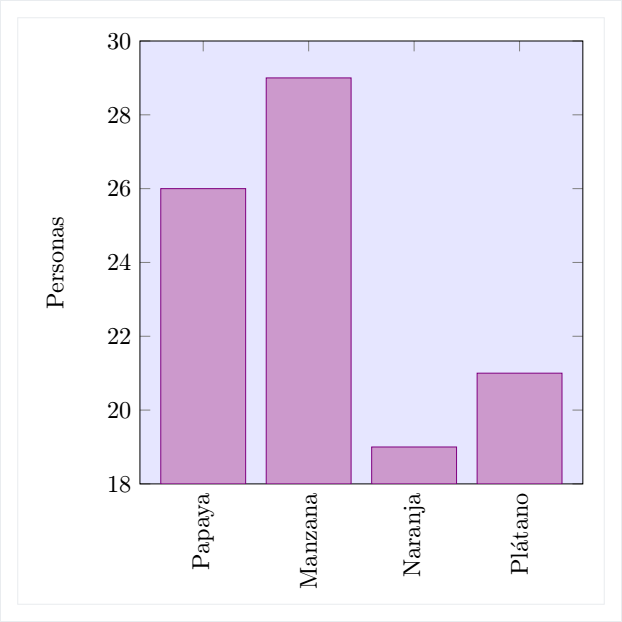
\includegraphics[width=\linewidth]{../images/imagen_barras_frutas01.png}
			\end{parts}
		\end{multicols}

	}

	\questionboxed[2]{Los resultados de una encuesta se muestran en la siguiente gráfica de barras:

		\begin{multicols}{2}
			\begin{parts}\normalsize
				\part ¿Cuántas personas participaron en la encuesta? \fillin[70][1.5cm]
				\part  ¿Cuál es la fruta menos preferida por las personas? \fillin[papaya][1.5cm]
				\part  ¿Cuál es la fruta preferida por las personas? \fillin[plátano][1.5cm]
				\part ¿Cuántas personas prefieren a las \textit{manzanas}.\fillin[16][1.5cm]
				\part ¿Cuántas personas prefieren a los \textit{plátanos}.\fillin[21][1.5cm]
				\part ¿Cuántas personas prefieren a las \textit{naranjas}.\fillin[19][1.5cm]

				\columnbreak%

				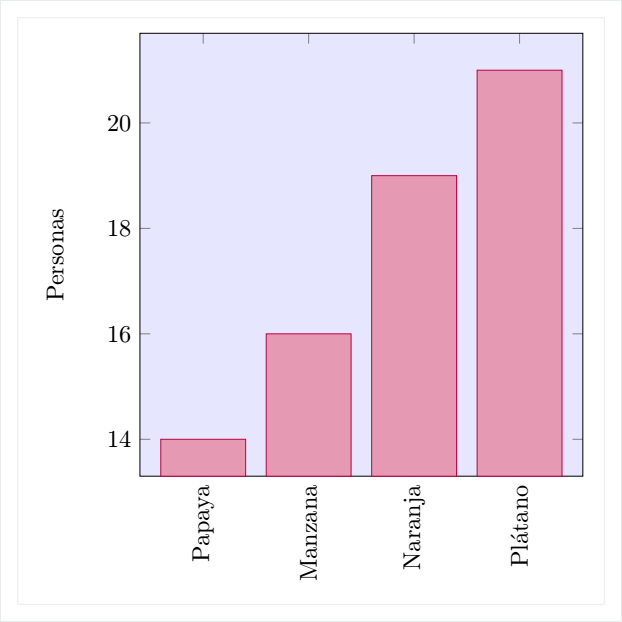
\includegraphics[width=\linewidth]{../images/imagen_barras_frutas02.png}
			\end{parts}
		\end{multicols}
	}


	% \subsection*{\ifprintanswers{Tablas de variación                }

	\questionboxed[2]{Contesta las siguientes preguntas:

		\begin{multicols}{2}
			\begin{parts}
				\part En la siguiente tabla se muestran la cantidad de personas que hay en aulas de una escuela. Si la cantidad de personas se mantienen constante, ¿cuántas personas habrá en 10 aulas?

				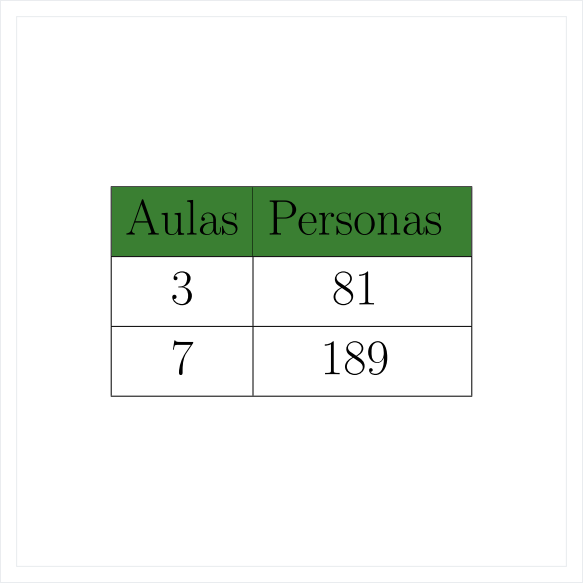
\includegraphics[width=0.45\linewidth]{../images/imagen_tabla_var06.png}
				\fillin[270][1.5cm]

				\part Con la información de la siguiente tabla, ¿cuál es el valor de x?

				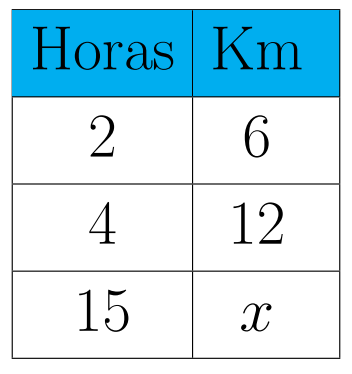
\includegraphics[width=0.35\linewidth]{../images/imagen_tabla_var03.png}
				\fillin[45][1.5cm]

				\part En la siguiente tabla se muestra el sueldo de una persona por hora trabajada. Si el pago se mantiene constante, ¿cuánto dinero recibe esta persona por hora trabajada?

				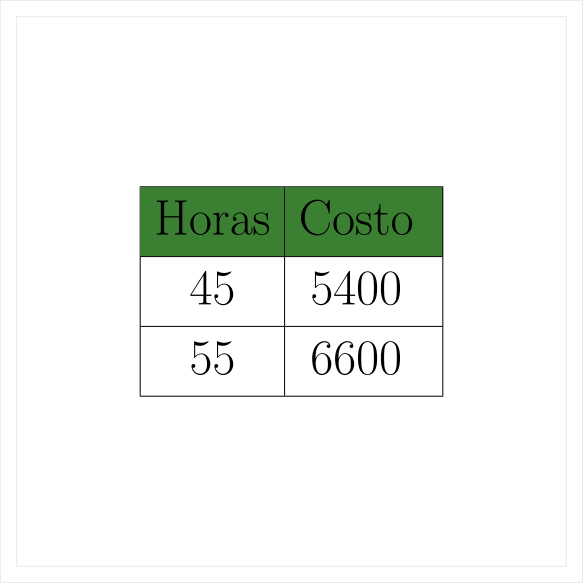
\includegraphics[width=0.4\linewidth]{../images/imagen_tabla_var05.png}
				\fillin[120][1.5cm]

				\part Con la información de la siguiente tabla, ¿cuál es el valor de x?

				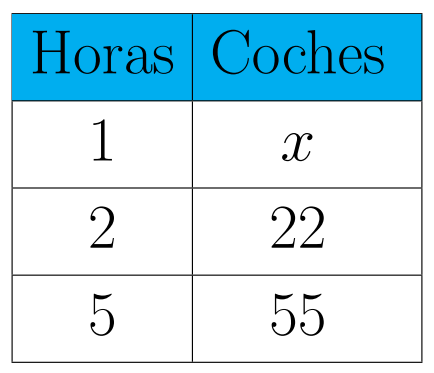
\includegraphics[width=0.42\linewidth]{../images/imagen_tabla_var04.png}
				\fillin[11][1.5cm]
			\end{parts}
		\end{multicols}
	}


	\addcontentsline{toc}{subsection}{Círculo}
	\subsection*{Círculo}
	% \subsection*{\ifprintanswers{Diámetro de un círculo             }
	% \subsection*{\ifprintanswers{Radio de un círculo                }
	\questionboxed[2]{Contesta las siguientes preguntas:

		\begin{multicols}{2}
			\begin{parts}
				\part ¿Cuál es el diámetro de un círculo que tiene un radio de 21.98?

				\begin{solutionbox}{1cm}
					\fillin[43.96][0cm]
				\end{solutionbox}

				\part ¿Cuál es el diámetro de un círculo que tiene un radio de 39.21?

				\begin{solutionbox}{1cm}
					\fillin[78.42][0cm]
				\end{solutionbox}

				\part ¿Cuál es el diámetro de un círculo que tiene un radio de 6.7?

				\begin{solutionbox}{1cm}
					\fillin[13.4][0cm]
				\end{solutionbox}

				\part ¿Cuál es el radio de un círculo que tiene un diámetro de 88.28?

				\begin{solutionbox}{1cm}
					\fillin[44.19][0cm]
				\end{solutionbox}

			\end{parts}
		\end{multicols}
	}

	% \subsection*{\ifprintanswers{Perímetro de un círculo            }
	% \subsection*{\ifprintanswers{Área de un círculo                 }

	\questionboxed[2]{Calcula el perímetro y área de los siguientes círculos:

		\begin{multicols}{3}
			\begin{parts}

				\part 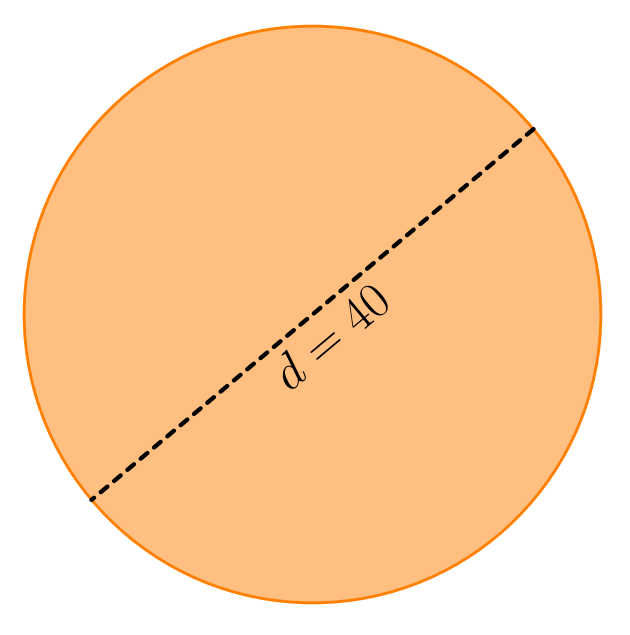
\includegraphics[width=0.8\linewidth]{../images/circulo01.png}\\
				\small Perímetro: \fillin[62.8][0.3in]  Área: \fillin[1256][0.3in]

				\begin{solutionbox}{1.2cm}\footnotesize
					% $P=8\pi=8(3.14)=25.12$ \\
					% $A=\pi(4)^2=3.14(4)^2=50.24$
				\end{solutionbox}

				\part 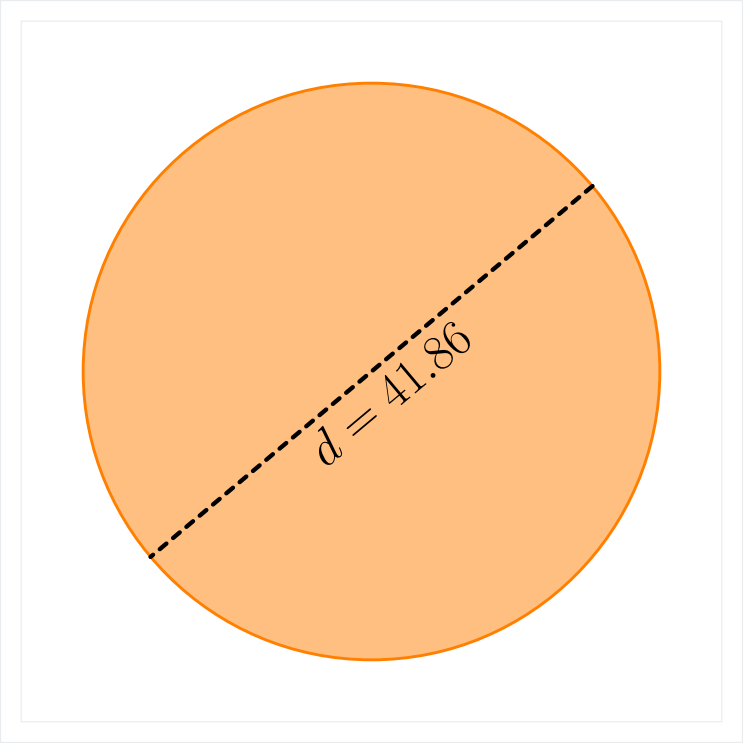
\includegraphics[width=0.8\linewidth]{../images/circulo02.png}\\
				\small Perímetro: \fillin[131.51][0.3in]  Área: \fillin[1376.22][0.3in]

				\begin{solutionbox}{1.2cm}\footnotesize
					% $P=2\pi r=2(3.14)(9.3)=58.4$ \\
					% $A=\pi r^2=3.14(9.3)^2=271.57$
				\end{solutionbox}

				\part 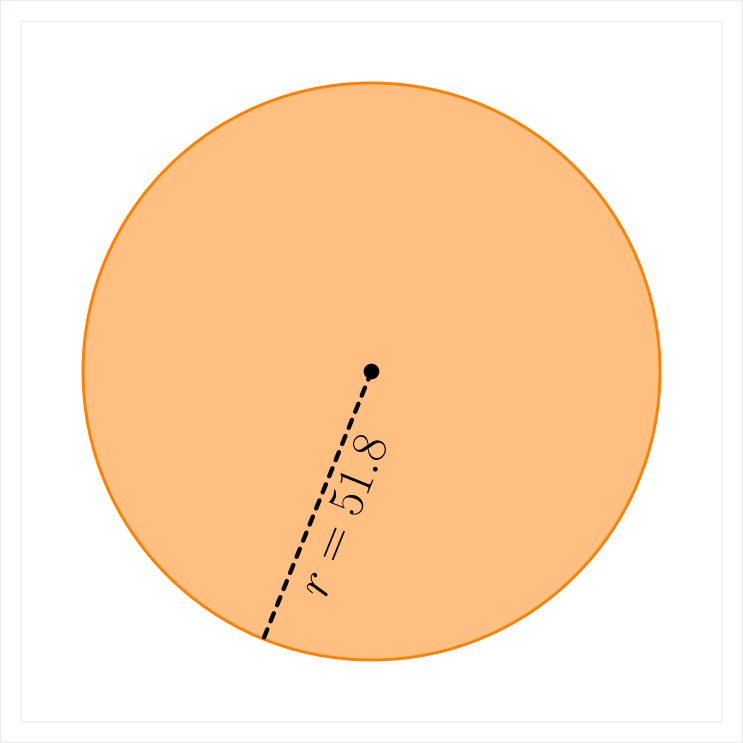
\includegraphics[width=0.8\linewidth]{../images/circulo03.png}\\
				\small Perímetro: \fillin[325.47][0.3in]  Área: \fillin[8429.65][0.3in]

				\begin{solutionbox}{1.2cm}\footnotesize
					% $P=2\pi r=2(3.14)(12)=75.36$ \\
					% $A=\pi r^2=3.14(12)^2=452.16$
				\end{solutionbox}

				\part 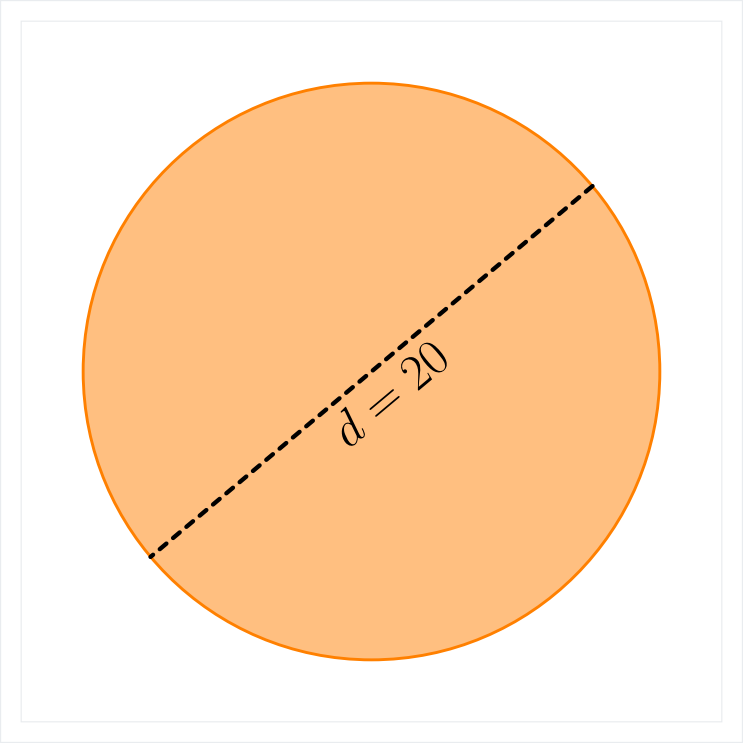
\includegraphics[width=0.8\linewidth]{../images/circulo04.png}\\
				\small Perímetro: \fillin[62.8][0.3in]  Área: \fillin[314][0.3in]

				\begin{solutionbox}{1.2cm}\footnotesize
					% $P=8\pi=8(3.14)=25.12$ \\
					% $A=\pi(4)^2=3.14(4)^2=50.24$
				\end{solutionbox}

				\part 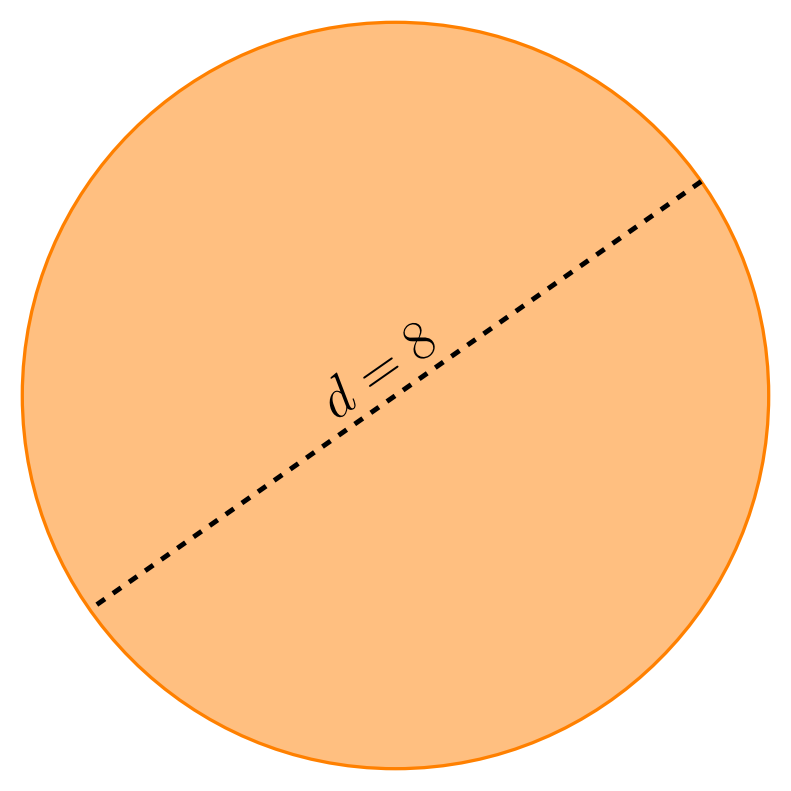
\includegraphics[width=0.8\linewidth]{../images/circulo05.png}\\
				\small Perímetro: \fillin[25.12][0.3in]  Área: \fillin[50.24][0.3in]

				\begin{solutionbox}{1.2cm}\footnotesize
					% $P=2\pi r=2(3.14)(9.3)=58.4$ \\
					% $A=\pi r^2=3.14(9.3)^2=271.57$
				\end{solutionbox}

				\part 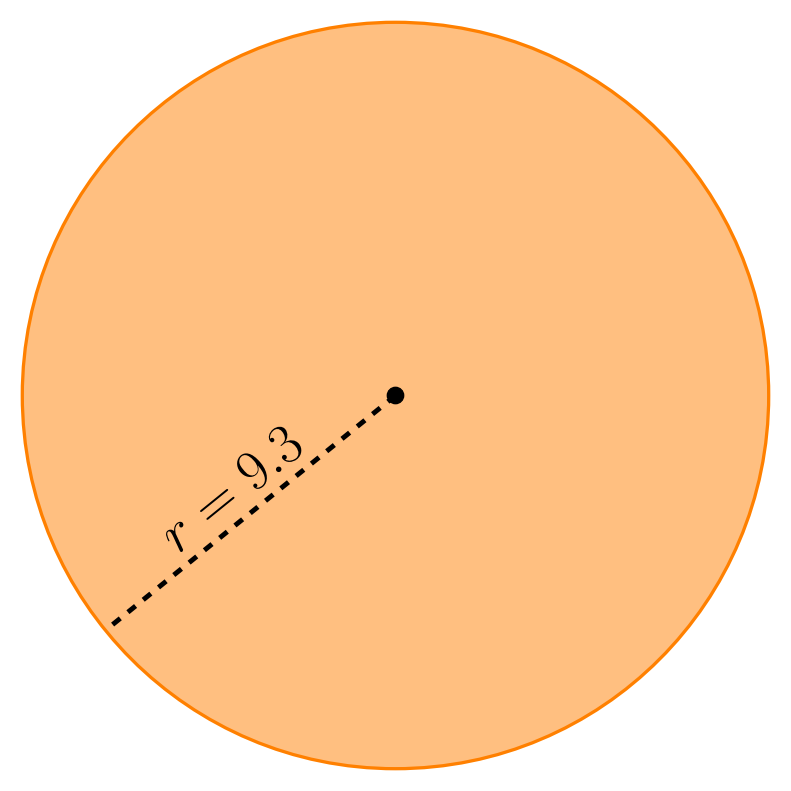
\includegraphics[width=0.8\linewidth]{../images/circulo06.png}\\
				\small Perímetro: \fillin[58.404][0.3in] Área: \fillin[271.57][0.3in]

				\begin{solutionbox}{1.2cm}\footnotesize
					% $P=2\pi r=2(3.14)(12)=75.36$ \\
					% $A=\pi r^2=3.14(12)^2=452.16$
				\end{solutionbox}
			\end{parts}
		\end{multicols}
	}





	% \subsection*{\ifprintanswers{Líneas del círculo                 }
	\addcontentsline{toc}{subsection}{Figuras geométricas}
	\subsection*{Figuras geométricas}

	% \subsection*{\ifprintanswers{Nombre de figuras                  }
	\questionboxed[2]{Escribe sobre la línea el nombre que recibe cada figura geométrica de acuerdo con su número de lados:

		\begin{multicols}{3}
			\begin{parts}
				\part 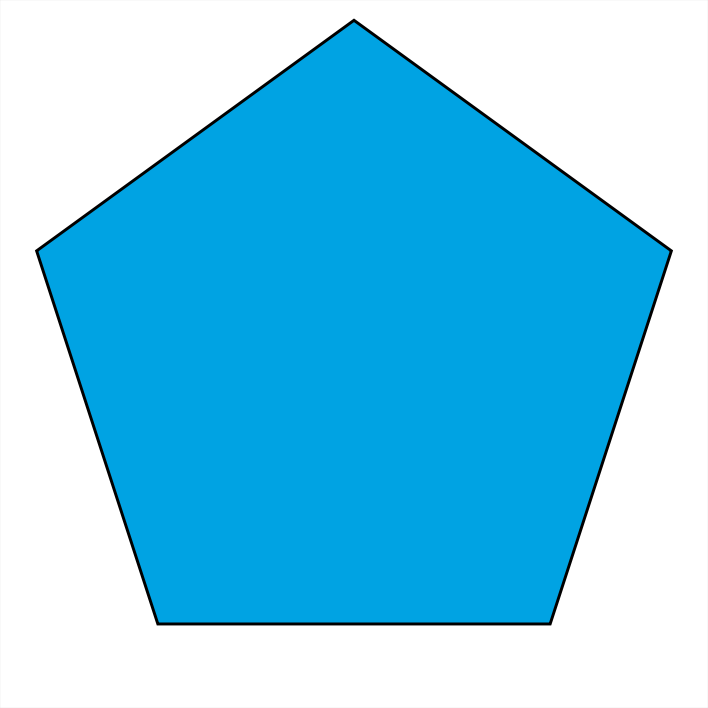
\includegraphics[width=75px]{../images/pentagono_azul.png}  \fillin[pentágono][0.75in]
				\part 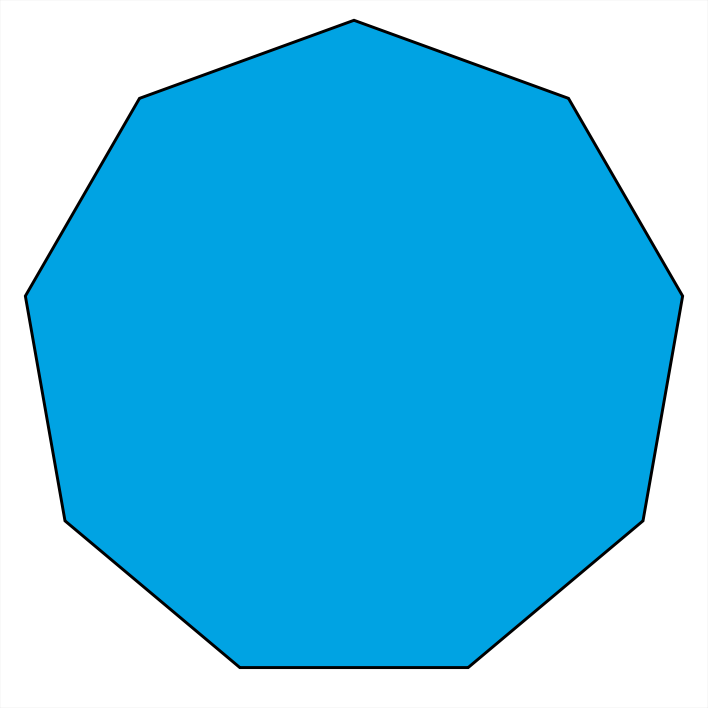
\includegraphics[width=75px]{../images/nonagono_azul.png}   \fillin[nonágono][0.75in]
				\part \includegraphics[width=75px]{../images/decagono_azul.png}   \fillin[decágono][0.75in]
				\part \includegraphics[width=75px]{../images/hexagono_azul.png}   \fillin[hexágono][0.75in]
				\part \includegraphics[width=75px]{../images/rectangulo_azul.png} \fillin[rectángulo][0.75in]
				\part \includegraphics[width=75px]{../images/cuadrado_azul.png}   \fillin[cuadrado][0.75in]
			\end{parts}
		\end{multicols}
	}


	% \subsection*{\ifprintanswers{Elementos de figuras               }
	% \subsection*{\ifprintanswers{Perímetro  }
	\questionboxed[4]{Contesta las preguntas sobre perímetros de figuras geométricas

		\begin{multicols}{2}
			\begin{parts}
				\part ¿Cuál es el perímetro de un rectángulo cuya base mide 38 y su altura mide 19?

				\begin{solutionbox}{1cm}
					\[P=38+19+38+19=\color{red}114\]
				\end{solutionbox}

				\part ¿Cuál es el perímetro de un cuadrado que sus lados miden 5?

				\begin{solutionbox}{1cm}
					\[P=5+5+5+5=\color{red}20\]
				\end{solutionbox}

				\part ¿Cuál es el perímetro de un pentágono que sus lados miden 18?

				\begin{solutionbox}{1cm}
					\[P=18 \times 5=\color{red}90\]
				\end{solutionbox}

				% \part ¿Cuál es el perímetro de un octágono que sus lados miden 15?

				% \begin{solutionbox}{1cm}
				% 	\[P=15 \times 8=\color{red}120\]
				% \end{solutionbox}

				\part ¿Cuál es el perímetro de un rombo que sus lados miden 16?

				\begin{solutionbox}{1cm}
					\[P=16 \times 4=\color{red}64\]
				\end{solutionbox}

			\end{parts}
		\end{multicols}
	}

	% \subsection*{\ifprintanswers{Área       }
	\questionboxed[2]{Contesta las preguntas sobre áreas de figuras geométricas

		\begin{multicols}{2}
			\begin{parts}
				\part ¿Cuál es el área de un triángulo cuya base mide 18 y su altura mide 11?

				\begin{solutionbox}{1.5cm}
					\[A=\dfrac{18 \times 11}{2}=\color{red}99\]
				\end{solutionbox}


				\part ¿Cuál es el área de un cuadrado que sus lados miden 29?

				\begin{solutionbox}{1.5cm}
					\[A=29 \times 29=\color{red}841\]
				\end{solutionbox}

			\end{parts}
		\end{multicols}
	}

	% \subsection*{\ifprintanswers{Resolución de problemas            }
	\addcontentsline{toc}{subsection}{Resolución de problemas}
	\subsection*{Resolución de problemas}
	% \subsection*{\ifprintanswers{Unidades de tiempo y reloj         }

	\questionboxed[2]{
		\begin{multicols}{2}
			\begin{parts}
				\part Convierte 23 horas a minutos:    \begin{solutionbox}{1cm}\fillin[1380][0in]\end{solutionbox}
				\part Convierte 27 horas a segundos:   \begin{solutionbox}{1cm}\fillin[97200][0in]\end{solutionbox}
				\part Convierte 3.9 horas a minutos:   \begin{solutionbox}{1cm}\fillin[234][0in]\end{solutionbox}
				\part Convierte 4.8 minutos a segundos:\begin{solutionbox}{1cm}\fillin[288][0in]\end{solutionbox}
			\end{parts}
		\end{multicols}
	}

	% \subsection*{\ifprintanswers{Cuerpos geométricos 1              }
	% \subsection*{\ifprintanswers{Cuerpos geométricos 2              }
	% \subsection*{\ifprintanswers{Resolución de problemas 1          }
	% \subsection*{\ifprintanswers{Resolución de problemas 2          }

	\questionboxed[2]{Resuelve los siguientes problemas:

		\begin{multicols}{2}
			\begin{parts}
				\part Alejandro quiere poner una barda alrededor de un terreno cuadrangular que mide 22 metros por lado. ¿Cuánta barda necesitará Alejandro para poner barda en todo el terreno?

				\begin{solutionbox}{1cm}
					\fillin[88][0in]
				\end{solutionbox}

				\part Para darle mantenimiento a una alberca olímpica se pone cinta alrededor de esta. Si la alberca tiene 50 metros de largo y 25 metros de ancho, ¿cuánta cinta se necesita para darle la vuelta a la alberca?

				\begin{solutionbox}{1cm}
					\fillin[150][0in]
				\end{solutionbox}


				\part Bruno corre todos los días en un parque de forma rectangular el cual mide 75 metros de largo y 40 metros de ancho. ¿Cuántos metros corre Bruno por una vuelta?

				\begin{solutionbox}{1cm}
					\fillin[230][0in]
				\end{solutionbox}

				\part Bruno corre todos los días en un parque de forma rectangular el cual mide 50 metros de largo y 28 metros de ancho. Si al día le da 4 vueltas al parque, ¿cuántos metros habrá corrido en total Bruno?

				\begin{solutionbox}{1cm}
					\fillin[624][0in]
				\end{solutionbox}
			\end{parts}
		\end{multicols}
	}

	\addcontentsline{toc}{subsection}{Sistema de unidades}
	\subsection*{Sistema de unidades}
	% \subsection*{\ifprintanswers{Multiplicaciones por múltiplos de 10}
	% \subsection*{\ifprintanswers{Divisiones por múltiplos de 10     }
	% \subsection*{\ifprintanswers{Unidades de longitud               }
	% \subsection*{\ifprintanswers{Unidades de masa                   }
	% \subsection*{\ifprintanswers{Unidades de capacidad              }
	\questionboxed[2]{Realiza las siguientes operaciones:

		\begin{multicols}{2}
			\begin{parts}
				% \part $ 93.2 \times 1000=$   \fillin[93200][0.5in]
				\part $ 84.2 \times 100=$   \fillin[8420][0.5in]
				\part $ 66.472 \times 10000=$   \fillin[664720][0.5in]
				\part $ 192.3 \times 10=$   \fillin[1923][0.5in]
				\part $ 26.9 \times 1000=$   \fillin[26900][0.5in]
				\part $ 81.674 \times 100000=$   \fillin[8167400][0.5in]
				\part $ 1.2 \times 1000=$   \fillin[1200][0.5in]
				\part $ 7.8 \times 10=$   \fillin[78][0.5in]
				\part $ 38093 \divisionsymbol 10=$   \fillin[3809.3][0.5in]
				\part $ 28 \divisionsymbol 1000=$   \fillin[0.028][0.5in]
				\part $ 44567 \divisionsymbol 100=$   \fillin[445.67][0.5in]
				\part $ 678 \divisionsymbol 1000=$   \fillin[0.678][0.5in]
				\part $ 7.1 \divisionsymbol 10=$   \fillin[0.71][0.5in]
				\part $ 51 \divisionsymbol 100=$   \fillin[0.51][0.5in]
				\part $ 3.9 \divisionsymbol 100=$   \fillin[0.039][0.5in]
				% \part $ 2.4 \divisionsymbol 100=$   \fillin[0.024][0.5in]
				% \part $ 34 \divisionsymbol 10=$   \fillin[3.4][0.5in]
				% \part $ 6.3 \divisionsymbol 10000=$   \fillin[0.00063][0.5in]
			\end{parts}
		\end{multicols}
	}




	\questionboxed[4]{Realiza las siguientes conversiones de unidades de longitud y masa:

		\begin{multicols}{2}
			\begin{parts}\normalsize
				\part De 157 kilómetros a hectómetros. \hfill \fillin[1570][0.6in] hm
				\part De 25 centímetros a milímetros.  \hfill \fillin[250][0.6in] mm
				\part De 27 kilómetros a decámetros.   \hfill \fillin[2700][0.6in] Dm
				\part De 17 kilómetros a hectómetros.  \hfill \fillin[170][0.6in] hm
				\part De 69 kilómetros a centímetros.  \hfill \fillin[6900000][0.6in] cm
				\part De 59 decímetros a centímetros.  \hfill \fillin[590][0.6in] cm
				\part De 26 metros a decímetros.       \hfill \fillin[260][0.6in] dm
				\part De 4 kilómetros a milímetros.    \hfill \fillin[4000000][0.6in] mm
				\part De 135 kilómetros a decámetros.  \hfill \fillin[13500][0.6in] Dm
				\part De 112 kilómetros a hectómetros. \hfill \fillin[1120][0.6in] hm
				\part De 205 gramos a decigramos    \hfill \fillin[2050][0.5in] dg
				\part De 25 kilogramos a gramos     \hfill \fillin[25000][0.5in] g
				\part De 58 kilogramos a gramos     \hfill \fillin[58000][0.5in] g
				\part De 45 decagramos a gramos     \hfill \fillin[450][0.5in] g
				\part De 134 gramos a decigramos    \hfill \fillin[1340][0.5in] dg
				\part De 282 gramos a miligramos    \hfill \fillin[282000][0.5in] mg
				\part De 117 decagramos a gramos    \hfill \fillin[1170][0.5in] g
				\part De 17 decigramos a miligramos \hfill \fillin[1700][0.5in] mg
				\part De 115 gramos a centigramos   \hfill \fillin[11500][0.5in] cg
				\part De 62 gramos a miligramos     \hfill \fillin[62000][0.5in] mg
			\end{parts}
		\end{multicols}
	}


	
\end{questions}
\end{document}